%%%%%%%%% MASTER -- compiles the 4 sections

\documentclass[10pt,letterpaper]{article}

%%%%%%%%%%%%%%%%%%%%%%%%%%%%%%%%%%%%%%%%%%%%%%%%%%%%%%%%%%%%%%%%%%%%%%%%%
\pagestyle{plain}                                                      %%
%%%%%%%%%% EXACT 1in MARGINS %%%%%%%                                   %%
\setlength{\textwidth}{6.5in}     %%                                   %%
\setlength{\oddsidemargin}{0in}   %% (It is recommended that you       %%
\setlength{\evensidemargin}{0in}  %%  not change these parameters,     %%
\setlength{\textheight}{8.5in}    %%  at the risk of having your       %%
\setlength{\topmargin}{0in}       %%  proposal dismissed on the basis  %%
\setlength{\headheight}{-40pt}      %%  of incorrect formatting!!!)      %%
\setlength{\headsep}{65pt}         %%                                   %%
\setlength{\footskip}{0.3in}       %%                                   %%
%%%%%%%%%%%%%%%%%%%%%%%%%%%%%%%%%%%%                                   %%
\newcommand{\required}[1]{\section*{\hfil #1\hfil}}                    %%
\renewcommand{\refname}{\hfil References Cited\hfil}                   %%
\bibliographystyle{plain}                                              %%
%%%%%%%%%%%%%%%%%%%%%%%%%%%%%%%%%%%%%%%%%%%%%%%%%%%%%%%%%%%%%%%%%%%%%%%%%

%PUT YOUR MACROS HERE

\usepackage{hyphenat}
\usepackage{layout}

\usepackage{verbatim} 
\usepackage{cite}
\usepackage[pdftex]{graphicx}
\usepackage{setspace}
\usepackage[cmex10]{amsmath}
\usepackage{amsmath, amsthm, amssymb}
\usepackage{algorithmic}
\usepackage{algorithm}

\usepackage{subfig}
\usepackage{caption}

%\usepackage[caption=false]{subfig}

%\usepackage{subcaption}
%\captionsetup{compatibility=false}

\usepackage{mathpazo}

\linespread{1.05}      % Palatino needs more leading (space between lines)

\usepackage{euler}

\usepackage{url}

%\usepackage{courier}
%\renewcommand{\familydefault}{\sfdefault}

%\usepackage[compact]{titlesec}
%\addtolength{\itemsep}{-0.05in}
%\usepackage{subcaption}
\usepackage{paralist}

\usepackage{tikz}

\usepackage{pgfplots}
% options for pgfplots
\pgfplotsset{compat=1.8,compat/show suggested version=false}
\usetikzlibrary{calc,trees,arrows,patterns,plotmarks,shapes,snakes,er,3d,automata,backgrounds,topaths,decorations.pathmorphing,decorations.markings}
%\pgfplotsset{compat=newest}
\pgfplotsset{
   /pgfplots/bar  cycle  list/.style={/pgfplots/cycle  list={%
        {black,fill=black!30!white,mark=none},%
        {black,fill=red!30!white,mark=none},%
        {black,fill=green!30!white,mark=none},%
        {black,fill=yellow!30!white,mark=none},%
        {black,fill=brown!30!white,mark=none},%
     }
   },
}
\usetikzlibrary{external}
\tikzexternalize[prefix=out/]
\tikzexternalize
% don't externalize todonotes
%\makeatletter
%\renewcommand{\todo}[2][]{\tikzexternaldisable\@todo[#1]{#2}\tikzexternalenable}
%\makeatother
% end of externalization
\usetikzlibrary{patterns}
\usepgfplotslibrary{groupplots}
\pgfplotsset{
every axis label/.append style={font=\footnotesize},
tick label style={font=\footnotesize},
}
%\usepackage[normalem]{ulem}
%\setlength{\abovecaptionskip}{2pt plus 2pt minus 2pt}
%\setlist{noitemsep,topsep=0pt}

\usepackage{wrapfig}

\usepackage[utf8]{inputenc}


%---------------------------------------------------------------------------------%
%*********************************************************************************%
%---------------------------------------------------------------------------------%


\title{\textbf{CSR:Small:Exploring Timing-Energy Tradeoffs on Heterogeneous Computing Platforms}}


\def\changemargin#1#2{\list{}{\rightmargin#2\leftmargin#1}\item[]}
\let\endchangemargin=\endlist

\hyphenation{op-tical net-works semi-conduc-tor}

%\pagestyle{fancy}
%\includeonly{NSFsumm}

\date{\vspace{4mm}}

%\doublespace

\begin{document}

%\layout

\maketitle
\pagenumbering{arabic}


%---------------------------------------------------------------------------------%
%*********************************************************************************%
%---------------------------------------------------------------------------------%
\newpage 

\begin{center}
\Large{\textbf{Project Summary}}
\end{center}

\paragraph{Summary.}

\paragraph{Intellectual merit.} 

\paragraph{Broader impacts.}

\paragraph{Keywords:} 

%---------------------------------------------------------------------------------%
%*********************************************************************************%
%---------------------------------------------------------------------------------%
\newpage 

\section{Introduction}
\label{sec:intro}

Recently, the microprocessor industry has adopted heterogeneous
multi-core processor designs for embedded systems. Heterogeneous
multicores integrate slow, lower-power cores with powerful and
power-hungry ones, to provide a wide range of power and performance
tradeoffs. Such heterogeneous computing platforms are seeing
widespread adoption in many cyber-physical systems (CPS) --- computing
systems that closely interact with the physical world --- including
intelligent automotive systems, medical devices, and smart robotics.
For example, the ARM big.LITTLE, which is a heterogeneous computing
architecture integrating relatively slow and fast cores, is expected
to see widespread adoption in automotive systems~\cite{armvehicle,
  armvehicle1, armvehicle2, armvehicle3}. This heterogeneous computing
technology can serve multiple automotive needs including infotainment
and advanced driver assistance systems. Succinctly, this processor
design has the potential to ``deliver exceptional power and
performance that aligns to the vision of scalable solutions for
automotive customers~\cite{armvehicle}.''

\vspace{2mm} \noindent \textbf{Two Fundamentally Conflicting Goals of
  Heterogeneous Computing in CPS: Timing Correctness and Energy
  Guarantees.} When timing correctness (i.e., enabling timing
constraints to be analytically validated at design time) takes the
form of hard real-time constraints, timing and energy efficiency are
fundamentally in conflict \cite{conflict-book}. The conflict arises
because hard real-time guarantees require reserving resources
sufficient for worst case latency.  In contrast, energy efficiency
requires allocating resources that just meet the needs of the current
job.  Even when worst case resource allocation is coupled with
aggressive energy reduction (e.g., in the form of voltage scaling
\cite{Dudani2002} or sleep states \cite{Huang2009}), this strategy is
less energy-efficient than allocating for the current case --- a fact
which has been demonstrated both analytically
\cite{Albers2011,Bansal2011,Irani} and empirically
\cite{LeSueur11,HotPower,Imes2014a,PowerSlope}. Of course, hard timing
guarantees are a requirement for correct operation of
CPS,\footnote{The functional correctness of most CPS hinges crucially
  upon the temporal correctness, as the control operations depend on
  the processing of certain environmental sensing and computation
  tasks} and their strict size, weight, and power (SWaP) requirements
-- as well as common reliance on battery power -- demand low energy
consumption.

\vspace{2mm} \noindent \textbf{Proposed approach.} Establishing timing
correctness requires real-time resource allocation methods. Most
existing works on real-time resource allocation in heterogeneous
systems focus on guaranteeing timing correctness (e.g., see
\cite{raravi2014task, raravi2013assigning, niemeier2011partitioned}
for an overview).  A couple of recently conducted
works~\cite{liuenergy, colin2014energy} seek to explore timing-energy
tradeoffs when designing resource allocation methods for heterogeneous
systems.  Unfortunately, such works fail to maximize energy efficiency
for two reasons. First, they have primarily focused on porting
existing techniques developed for homogeneous systems, i.e., they make
scheduling decisions based purely on timing-related concerns and then
reduce energy consumption on a ``best-effort'' basis.  When ported to
heterogeneous systems, existing techniques are more energy efficient,
but this gain is entirely due to the processor architecture and not an
inherent feature of the algorithm. The key insight in our proposed
work will be to start from scratch and incorporate knowledge of
heterogeneity and energy into our proposed algorithms from the
beginning of the project.  This approach promises to lead to new
algorithms that have better energy efficiency and offer new
capabilities. Second, the existing works make the following critical
assumption: all processor cores can operate at max speed all the time
while sustaining safe power dissipation.  This assumption is
unfortunately invalid due to the critical ``dark silicon'' effect;
i.e., essentially all processors are over-provisioned and have much
larger maximum compute capacity than they can safely
sustain\cite{exynos5,DaSi2011,Venkatesh2010}. Motivated by these
observations, our goal is to simultaneously achieve timing correctness
and energy efficiency on heterogeneous platforms by:
\textbf{(\textit{i}) identifying the most energy-efficient resource
  allocation methods that guarantee timing correctness on a
  heterogeneous platform}, and \textbf{(\textit{ii}) developing
  aggressive energy-oriented resource allocation methods that exploit
  dark silicon, where heterogeneous processors have tremendous
  additional compute capacity that can only be used for short amounts
  of time}. Such methods would aggressively achieve significant energy
savings while avoiding timing errors by utilizing the over-provisioned
processing capacity in short bursts.


\vspace{2mm} \noindent \textbf{Research objectives.} We will pursue
the following four-step plan to accomplish our research goal.
\begin{itemize}\itemsep 0pt \parskip 0pt
\item \textbf{Step1: Identify the most energy-efficient configurations
    of resource allocation and DVFS that guarantee timing:} We will
  design energy-oriented scheduling methods for heterogeneous
  platforms. The goal is to minimize energy consumption while
  guarantee timing correctness. For each devised algorithm, formal
  timing validation tests will be developed.
\item \textbf{Step 2: Develop aggressive energy-saving techniques that
    exploit dark silicon.}  We will develop new resource allocation
  techniques that aggressively reduce energy consumption for mixed
  critical real-time workloads by spending as much time as possible in
  slower, more energy-efficient states. Timing errors will be avoided
  by utilizing the over-provisioned processing capacity in short
  bursts.
\item \textbf{Step 3: Carry out overhead-aware schedulability
    studies.} The research in the first two steps will provide
  solutions for simultaneously achieving timing correctness and energy
  guarantees on heterogeneous computing platforms. To evaluate their
  effectiveness in practice, we will incorporate them in real hardware
  (based on the ARM big.LITTLE architecture) and conduct large-scale
  overhead-aware schedulability experiments with both synthetic
  workloads with widely varied parameters and benchmarks.  We plan to
  apply an extensive methodology that is designed for comparing
  real-time resource allocation strategies in an overhead-cognizant
  way \cite{clustered, bastoni2010, BBBdissertation}, which is proven
  to be effective for many real-time systems.
\item \textbf{Step 4: Conduct case-studies.} To determine if our
  proposed methods can be applied in practice, we intend to conduct
  case-study evaluations using several specific real-time workloads
  seen in automotive systems. For example, one such application we
  will consider is real-time object recognition, which is heavily
  performed in automotive systems for implementing tools such as
  collision avoidance and traffic sign recognition. We will evaluate
  the performance in terms of several specific metrics for using one
  or more preferable configurations identified in Step~3 to support
  such workloads.
\end{itemize}

\vspace{2mm} \noindent \textbf{Qualification.} The PIs are
well-qualified to conduct this research. The proposing team has worked
on various aspects of real-time systems, heterogeneous multicore
computing, and energy optimization in the past years, including
theoretical real-time analysis~\cite{Liu1, Liu2, Liu6, Liu7, Liu10,
  liu2014supporting, Liu3, Liu4, Liu5, Liu9, Liu11, Liu13,
  chen2015k2u}, real-time operating systems~\cite{elliott1minimizing,
  Liu12, GPES, zhou2015supporting, Zhou2014a}, heterogeneous multicore
architecture~\cite{Zhou2014a, GPES}, and energy efficient computing
under various computer architectures~\cite{Liu12}. These efforts have
resulted in a number of publications accepted by several systems- and
architecture-related premium conference and journal venues such as
SOSP, ASPLOS, RTSS, ISCA, Micro, and IEEE Transactions on Parallel and
Distributed Systems.  PI Liu has been working on developing device
driver and operating systems support for heterogeneous real-time
systems~\cite{GPES, zhou2015supporting, Zhou2014a}, resource
allocation on heterogeneous platforms~\cite{Tong14a, LiuRTSS14a,
  chen2015k2u, Liu12, elliott1minimizing}, and real-time
schedulability analysis~\cite{Liu1, Liu2, Liu6, Liu7, Liu10,
  liu2014supporting, LiuRTSS14b, Liu3, Liu4, Liu5, Liu9, Liu11,
  Liu13}.  PI Hoffmann at the University of Chicago has rich experience
in homogeneous\cite{raw1,raw2,raw3,tilera1,tilera2} and
heterogeneous \cite{ASAP,HPEC,ASAP2,ISSoC} processor design as well
as operating systems support for managing performance and power
tradeoffs
\cite{LEO,POET,DynamicKnobs,JouleGuard,PTRADE,PCP,TCST,HotPower,kim-cpsna}.


%*********************************************************************************%
%*********************************************************************************%

\section{Background and Related Work}
\label{sec:motivation}
<<<<<<< HEAD
In this section, we first describe the heterogeneous computing architecture and the associated energy and performance characteristics of such platforms. ARM's big.LITTLE will be used as an example heterogeneous computing platform we choose to focus in this document. To ensure timing correctness, real-time resource allocation techniques must be used. We will thus discuss traditional real-time scheduling-related terminology and workload models. Finally, we describe the experimental platform to be used in our research. Due to space constraints, our overview of prior work focuses on research of direct relevance to our agenda.
=======
This section motivates the need for the proposed research.  We first
illustrate how the emergence of heterogeneous single-ISA architectures
and dark silicon change timing and energy tradeoffs making previously
useful resource allocation strategies extremely inefficient.  We then
discuss background in real-time scheduling and schedulability.
Finally, we discuss related work scheduling for heterogenous systems.
\emph{Critically, we find that prior work has not...}
>>>>>>> 13d73883f1b0cb55eabc89896f2e4ce55936aaf0


%*********************************************************************************%

\subsection{Hardware Platform}
\label{sec:hardware}
 
\subsubsection{Architecture Trends}
Modern computing systems are constrained by \emph{dark silicon};
\emph{i.e.}, not all transistors can be powered at all times
\cite{DaSi2011,Venkatesh2010}.  The emergence of dark silicon has led
hardware architects to rethink processor design.  Recent designs
incorporate differing cores with a common instruction set and
programming model~\cite{Kumar.2005.heterogeneous,SulemanMQP09}.  Some
cores are complex with deep pipelines and large issue width, while
others are much simpler \cite{bigLittle}.  These \emph{heterogeneous
single-ISA} designs improve energy efficiency by executing computation
on the most appropriate type of core.

While these processors present a wide range of performance and energy
tradeoffs, they create a difficult scheduling problem.  Not only, does
a software scheduler have to map tasks to core types, it also most
ensure that energy is minimized (to increase battery life) and that
critical power threshholds are not violated.  For example, the Exynos
5 processor (based on an ARM big.LITTLE architecture \cite{bigLittle})
has a 5.5W peak power that is nearly $2 \times$ the maximum
sustainable heat dissipation, limiting peak speed to less than 1
second \cite{exynos5}.  In addition, our prior work has shown that
this processor achieves greater energy efficiency as it slows down
\cite{Imes2014}.  

Such a processor desing creates both a challenge and an opportunity
for real-time embedded processing. The challenge is how to ensure that
timing constraints are met while operating in the most
energy-efficient configuration.  The opportunity comes from the fact
that the processor is overprovisioned, it has a much higher compute
capacity than it can safely sustain.  This extra compute capacity
could be used in short bursts to prevent timing errors.  The next
section illustrates these concepts with empirical results.

\subsubsection{Preliminary Results}

\begin{table*}[th]
\caption{Two embedded platforms with different configurable components.}
\label{tbl:machines}
\scriptsize 
\centering
\begin{tabular}{lcccccccc}
  \textbf{Type} & 
  \textbf{Processor} &
  \textbf{Cores} & 
  \textbf{Core Types} &
  \textbf{Speeds (GHz)} &
  \textbf{TurboBoost} &
  \textbf{HyperThreads} & 
  \textbf{Idle Power (W)} & 
  \textbf{Configurations} \\
  \hline
  \hline
  Homogeneous   & Intel Haswell Mobile       & 2 & 1 & .6--1.5  & yes & yes & 2.5 & 45 \\
  Heterogeneous & Samsung Exynos5 Octa & 8 & 2 (A15 \& A7) & .8--1.6 (A15) .5-1.2 (A7) & no & no & 0.12 & 69 \\
  \hline 
  \hline
\end{tabular}
\vskip -.7em
\end{table*}

We use an example application to compare the different tradeoffs on a
heterogeneous single-ISA processor and a homogeneous multicore.  As a
target application, we use a video encoder, composed of jobs, where
each job encodes a frame. We instrument the encoder to report job
latency and measure each processor's energy consumption.  The two
processors have different configurable resources, shown in
Table~\ref{tbl:machines}.

\begin{figure}[t]
\vskip -1.8em
\subfloat[Energy/Latency Tradeoffs]%
{\begin{tikzpicture}
\begin{centering}


\definecolor{s1}{RGB}{228, 26, 28}
\definecolor{s2}{RGB}{55, 126, 184}
\definecolor{s3}{RGB}{77, 175, 74}
\definecolor{s4}{RGB}{152, 78, 163}
\definecolor{s5}{RGB}{255, 127, 0}

% \begin{groupplot}[
%     group style={
%         group name=plots-labeltop,
%         group size=2 by 1,
%         xlabels at=edge top,
%         xticklabels at=edge top,
%         vertical sep=5pt,
%     },
% xlabel near ticks,
% height=4cm,
% width=0.5\textwidth,
% xtick=\empty,
% ytick=\empty,
% xmin=0,
% xmax=20,
% ymin=0,
% ymax=1.5,
% ]
% \nextgroupplot[xlabel={\footnotesize $\mathsf{Performance}$ (normalized latency)}]
% \nextgroupplot[xlabel={\footnotesize $\mathsf{Power}$ (Watts)}]
% %\nextgroupplot[xlabel={\footnotesize $\mathsf{Accuracy}$}]
% %\nextgroupplot[]
% %\nextgroupplot[]
% %\nextgroupplot[]
% \end{groupplot}

\begin{groupplot}[
    group style={
        group name=plots,
        group size=1 by 1,
        xlabels at=edge bottom,
        xticklabels at=edge bottom,
        vertical sep=5pt
    },
xlabel={\footnotesize $Latency$ 
%(normalized to worst case)
},
xlabel near ticks,
height=3.5cm,
%width=0.5\textwidth,
width = 4.2cm,
xmajorgrids,
ymajorgrids,
grid style={dashed},
xtick={0,0.25,0.5,0.75,1.0},
xticklabels={0,0.25,0.5,0.75,1.0},
xticklabel style={font=\footnotesize},
xmin=0,
xmax=1.1,
yticklabel pos=left,
enlargelimits=false,
tick align = outside,
tick style={white},
xticklabel shift={-5pt},
yticklabel shift={-5pt},
ylabel shift={-2pt},
ylabel style={align=center},
unbounded coords=jump,
]

\nextgroupplot[ylabel={\footnotesize Energy}, 
%ylabel shift={6mm},
ytick={0,0.25,0.5,0.75,1.0},
yticklabels={0,0.25,0.5,0.75,1.0},
yticklabel style={font=\footnotesize},
ymin=0,
ymax=1.1,
legend entries={{\scriptsize $\mathsf{Vaio}$},{\scriptsize $\mathsf{ODROID}$}},
legend style={draw=none,at={(0.5,1.35)},anchor=north,legend columns=4,line width=5pt},
]
\addplot[thick, solid, color=s1, only marks, mark=square*] table[x index=2,y index=5,col sep=tab] {img/vaio-tradeoffs.txt};
\addplot[thick, solid, color=s3, only marks, mark=*] table[x index=2,y index=5,col sep=tab] {img/odroid-tradeoffs.txt};


\end{groupplot}
\end{centering}

\end{tikzpicture}
%
\label{fig:x264-motivation-tradeoffs}}
\subfloat[Energy Consumption]%
{\begin{tikzpicture}

\begin{groupplot}[
    group style={
        group name=plots,
        group size=1 by 1,
        xlabels at=edge top,
        xticklabels at=edge top,
        vertical sep=5pt
    },
axis x line* = top,
xlabel near ticks,
major x tick style = transparent,
height=3.5cm,
%width=0.95\columnwidth,
width=4.2cm,
xmin=0,
xmax=3,
enlargelimits=false,
tick align = outside,
tick style={white},
ytick=\empty,
xtick=\empty,
xticklabels={},
yticklabels={},
]
\nextgroupplot[ylabel={\footnotesize Energy},
ylabel shift={6mm},
ymin=0,
ymax=1,
]


\end{groupplot}

\begin{groupplot}[
    group style={
        group name=plots,
        group size=1 by 1,
        xlabels at=edge bottom,
        xticklabels at=edge bottom,
        vertical sep=5pt
    },
axis x line* = bottom,
xlabel near ticks,
major x tick style = transparent,
height=3.5cm,
%width=0.95\columnwidth,
width=4.2cm,
xmin=0,
xmax=3,
enlargelimits=false,
tick align = outside,
tick style={white},
ytick=\empty,
xticklabel shift={-5pt},
%x tick label style={rotate=0, anchor=south},
xlabel={\footnotesize $Platform$},xtick={1,2,3},
xticklabels={{\scriptsize $\mathsf{Vaio}$},
{\footnotesize $\mathsf{ODROID}$}},
ymin=1,
ymax=2.25,
ytick={1.0,1.25,1.5,1.75,2.0},
yticklabels={1.00,1.25,1.50,1.75,2.00,2.25},
legend cell align=left, 
legend style={ column sep=1ex },
ymajorgrids,
grid style={dashed},
]
\nextgroupplot[ybar=\pgflinewidth,
bar width=5pt,
legend entries = {{\scriptsize $\mathsf{never~idle}$},{\scriptsize $\mathsf{race~to~idle}$}},
legend style={draw=none,legend columns=2,at={(0.5,1.35)},anchor=north},
]
\addplot table[x index=0,y index=2, col sep=space] {img/heuristics2.txt};
\addplot table[x index=0,y index=3, col sep=space] {img/heuristics2.txt};


\end{groupplot}

\end{tikzpicture}
%
\label{fig:x264-motivation-heuristics}}
\caption{Energy/latency tradeoffs.}
\label{fig:x264-motivation}
\end{figure}

The different shapes of these tradeoff spaces lead to different
optimal resource allocation strategies. Empirical studies show that
the \emph{race~to~idle} heuristic, which makes all resources available
and then idles after completing a job, is near optimal on systems like
the homogeneous
processor~\cite{PowerSlope,Hoelzle2009,google,Imes2014,HotPower}.  On
systems like the heterogeneous processor, recent approaches save
energy by keeping the system constantly busy and
\emph{never~idle}~\cite{Carroll13,LeSueur11,Lin2010,Imes2014,HotPower}.

To demonstrate how different scheduling decisions affect the different
platforms, we compare the energy consumption of both race-to-idle and
never-idle.  We set a latency target equal to the worst observed
latency for this application on each processor and measure the energy
consumption of encoding 500 video frames using each heuristic.
Figure~\ref{x264-motivation-heuristics} shows the results, normalized to
the optimal energy found by measuring every possible resource
configuration for each frame.  Both heuristics meet the latency
target, but their energy consumptions vary tremendously. On the
homogeneous processor, \emph{race~to~idle} is near optimal, but
\emph{never~idle} consumes 13\% more energy.  Conversely,
\emph{never~idle} is near optimal for the heterogeneous processor, but
\emph{race~to~idle} consumes $2 \times$ more energy.

These results demonstrate two key points:
\begin{itemize}
\item The conventional approach of allocating all resources and
transitioning to a low power idle state is extremely inefficient on
the heterogeneous processor.  
\item The heterogeneous processor can
reach speeds of up to XX faster than it can safely sustain.
\end{itemize}


%*********************************************************************************%

\subsection{Real-Time Scheduling Algorithms and Schedulability Tests}
\label{sec:model}
The goal of real-time scheduling is to guarantee timing correctness; in other words, every task is schedulable if it meets the predefined timing constraints at design time. Being ``schedulable'' depends on whether task deadlines are hard or soft. %(We consider both possibilities in this research.) 
For a hard real-time (HRT) task, its deadline must be met; while for a soft real-time (SRT) task, missing some deadlines can be tolerated. %For example, in an automotive system, autonomous control and emergent collision avoidance  are  HRT tasks; while automatic lane following and traffic sign recognition can be viewed as SRT tasks. 
 SRT constraints can be defined in several ways. We assume a well-studied SRT notion \cite{mills2010stochastic, erickson2012soft, johndissertation, BBBdissertation, devidissertation, leontyevdissertation} that a SRT task is schedulable if its response time can be provably bounded. (Such bounds would be expected to be reasonably small.) In this research, we consider both HRT and SRT possibilities.  

To ensure timing predictability, we must develop two kinds of algorithms: \textit{real-time scheduling algorithms} and \textit{schedulability tests}. A scheduling algorithm (i.e., scheduler) determines when to execute which task and on which resource. Scheduling algorithms can usually be divided into two major categories: (\textit{i}) partitioning, and (\textit{ii}) global scheduling. %, and (\textit{iii}) clustered scheduling. 
Under partitioning, tasks are statically partitioned among processors~\cite{andersson2003, baker2007, funk2005, Baruah2006a, chattopadhyay2011, baruah2005a}. %; i.e., each task is bound to execute on a specific processor and will never migrate to another processor \cite{andersson2003, baker2007, funk2005, Baruah2006a, chattopadhyay2011, baruah2005a}. 
Different processors can apply different scheduling algorithms. A partitioning algorithm example is partitioned earliest-deadline-first (EDF), which uses the EDF algorithm as the per-processor scheduler. (Under EDF, jobs with earlier deadlines have higher priority.) In contrast to partitioning, under global scheduling, a single global ready queue is used for storing ready jobs \cite{baruah2008, bertogna2011b, BC, devi2005}. Jobs are allowed to migrate from one processor to another at any time. A global scheduling algorithm example is global EDF (GEDF), under which jobs are EDF-scheduled using a single ready queue. 
 Clustered scheduling is hybrid of partitioned and global scheduling in which tasks are statically assigned to a cluster of processors, among which the task can freely migrate.
 Note that the ARM's big.LITTLE platform we will focus in this research has implemented the general global and clustered scheduling policies. Moreover, under another categorization method of scheduling algorithms, we have two kinds of schedulers, fixed-priority and dynamic-priority schedulers, where a fixed-priority scheduler assigns a fixed priority to each task and all the jobs released by this task inherit the same task priority (e.g., rate-monotonic scheduling which assigns higher priorities to tasks with shorter periods) and a dynamic-priority scheduler assigns every job a different priority (e.g., EDF).
 
  %On multi- and many-core systems, clusters are often aligned to the underlying hardware architecture so as to prevent expensive migrations between remote cores. It has been shown that such migration overhead reductions could enhance the overall performance in embedded systems with stringent SWaP constraints (e.g., an automotive system)~\cite{bastoni2010}.

%It is executed repeatedly at runtime during the lifetime of a real-time system. 
Depending on the scheduling algorithm being used, at design time a corresponding schedulability test verifies whether a task system will be schedulable, provided that the system behaves according to its parameterized specification. Finding an optimal scheduling algorithm that experiences no capacity loss (i.e., 100\% resource utilization) is not always possible. If a non-optimal scheduling algorithm is used, then a schedulable task system may be deemed unschedulable by the corresponding schedulability test due to algorithmic capacity loss.
Our goal of designing energy-efficient scheduling algorithms and schedulability tests is to minimize the overall capacity loss.% (i.e., maximize resource utilization). 

%In practice, finding an optimal scheduling algorithm that can fully allocate all processor capacity to real-time tasks is not always possible.
%; i.e., task systems with total utilization less than $m$ may not be schedulable on $m$ processors. 
%One primary cause of such capacity loss is due to the choice of a scheduling algorithm. If a non-optimal scheduling algorithm is used, then a schedulable task system may be deemed unschedulable due to algorithmic capacity loss. Our goal of designing resource-conscious scheduling and schedulability analysis algorithms is to minimize the capacity loss on all resources (i.e., maximize resource utilization). 

\begin{comment}

\begin{wrapfigure}{r}{0.46\textwidth}
%	\captionsetup{width=0.65\textwidth}  
\vspace{-4mm}
	\begin{center}
          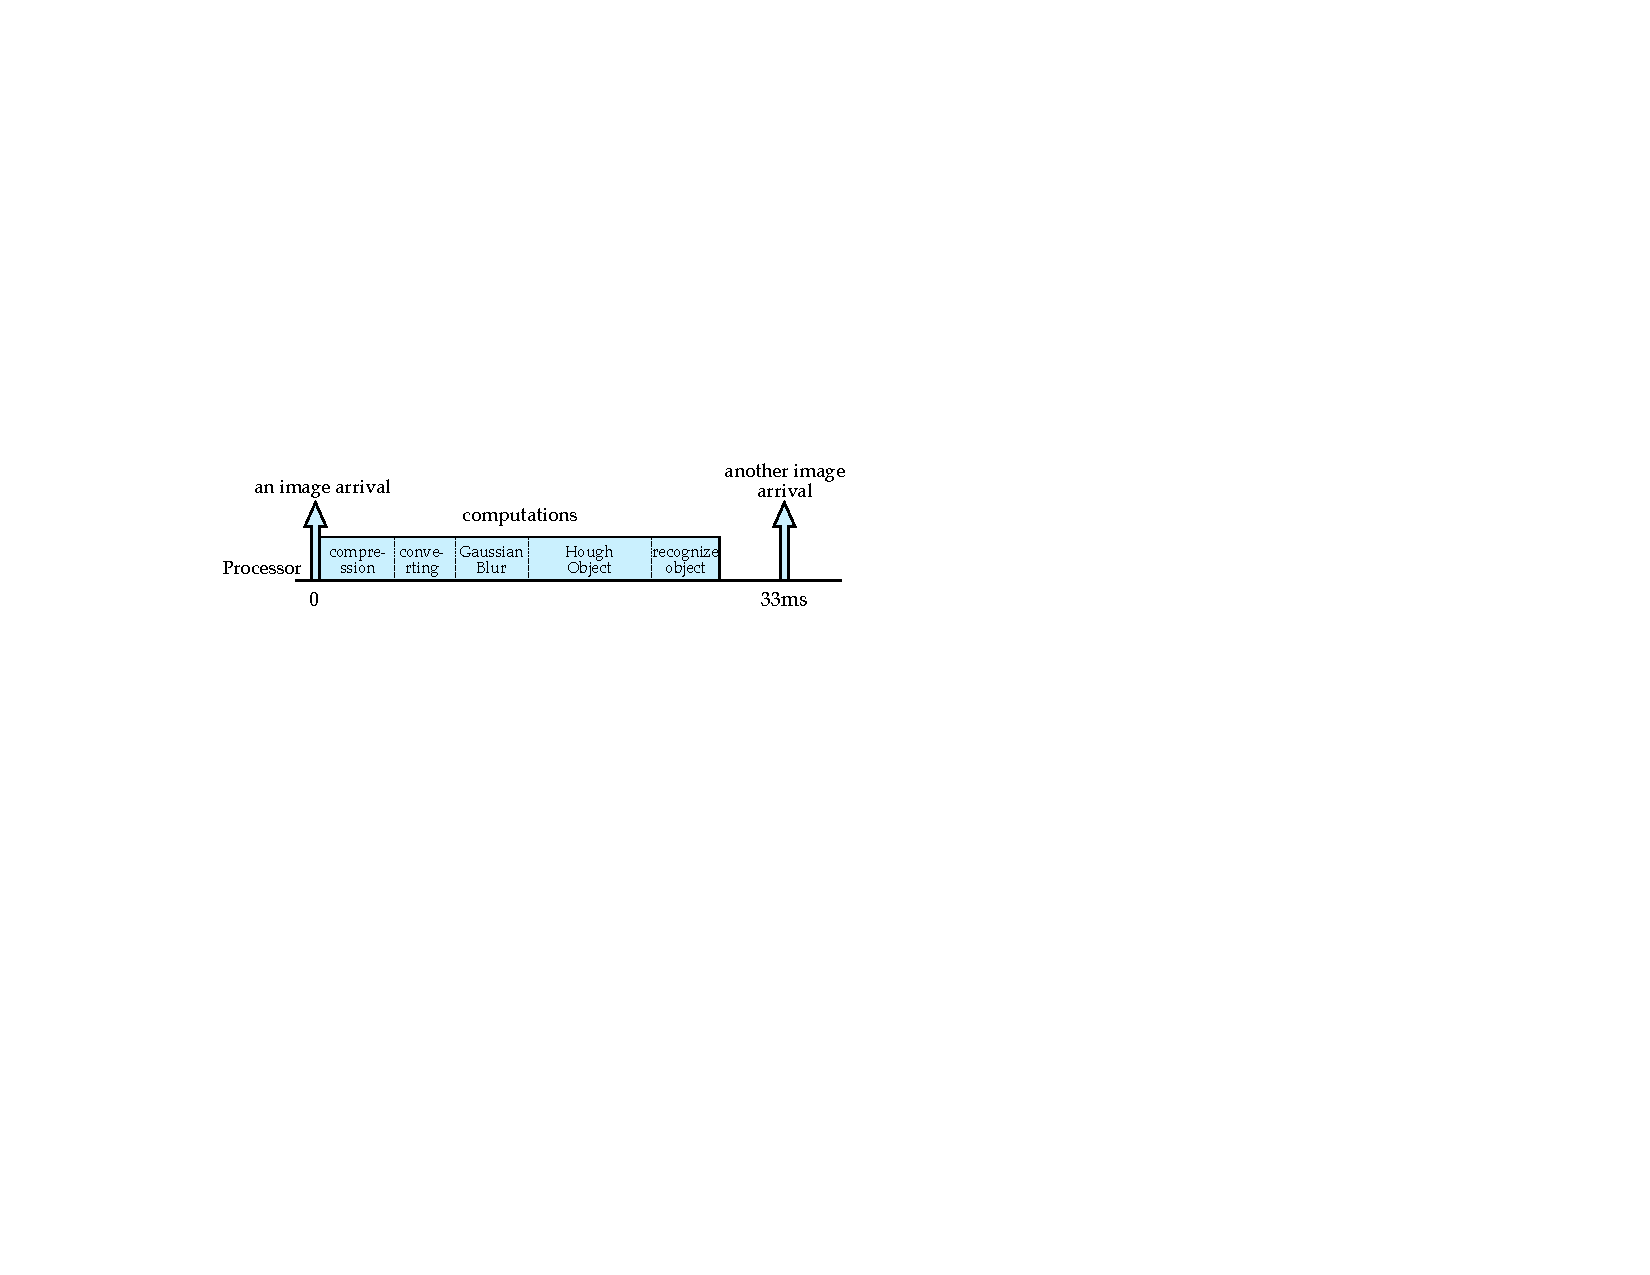
\includegraphics[width=3in]{images/sporadiceg.pdf} 
    \end{center}
    \vspace{-2mm}
\caption{\small The sporadic job releasing pattern of object recognition applications.}
\vspace{-2mm}   
\label{fig:sporadiceg}
\end{wrapfigure} \normalsize
\end{comment}

\paragraph{Workload Models.} Real-time embedded systems commonly perform recurring operations. For example, the object recognition application commonly involved in implementing many autonomous-driving assisted functionality is naturally recurrent. Specifically, the camera sensor captures an image at a certain frequency; each image is compressed and then analyzed using certain object recognition algorithms, and is expected to be completed by the invocation of the next frame; e.g., each invoked job ideally should complete the corresponding workloads within 33\textit{ms} for a 30 frame-per-second camera. %, as illustrated in Figure~\ref{fig:sporadiceg}.  

Generally speaking, a specified real-time system consists of a collection of recurring real-time processes called ``tasks''. %A real-time task is a  program that is repeatedly invoked in response to external events such as device interrupts or expiring timers. When a task is invoked in response to an event, it releases a ``job'' to process the event. 
A widely studied general model of recurrent workloads is the \textit{sporadic task model}~\cite{sporadic}. In this model, the specified system is composed of a collection of recurring\footnote{Although our focus in this document is on the notion of recurrence found in the sporadic model, we intend to consider other such notions in our work.} %Moreover, although recurrent task arrival pattern is dominant in real-time embedded systems, other patterns in practice may exist. As seen in Sec.~\ref{sec:remoteresource}, we will also consider other workload arrival patterns such as non-recurrent and independent jobs that often appear in the emerging mobile embedded systems.} 
sequential tasks, $\tau = \lbrace \tau_1$, ..., $\tau_n \rbrace$. Each such task $\tau_i$ releases a succession of \textit{jobs} $J_{i,1}$, $J_{i,2}$, ... and is defined by specifying a \textit{period} $T_i$, a \textit{relative deadline} $D_i$, and a \textit{worst-case execution time (WCET)} $C_i$. Successive jobs of $\tau_i$ are released at least $T_i$ time units apart, and one that is released at time $t$ has a deadline at time $t+D_i$. Also, each such job executes for at most $C_i$ time units. %Fig.~\ref{fig:modeleg}(b) shows an example sporadic task that models a simple control application.
Each job released by any task has a \textit{response time} that defines the duration from its release to its finish time. A task $\tau_i$'s response time equals the maximum job response time among all of its released jobs. 

%The sporadic task model has received an enormous amount of attention~\cite{andersson2003, baker2007, funk2005, Baruah2006a, chattopadhyay2011, baruah2005a, baruah2008, bertogna2011b, BC, baruah1996, goossens2003, baker2003, Cluster1, davis2011a, devi2005, baruah1996, baruah2007, G, Par}. Unfortunately, it assumes that CPU is the only computing resource in the system and thus cannot be used to model workloads that may access both CPU and GPU resources.

\begin{figure}[h]
\centering 
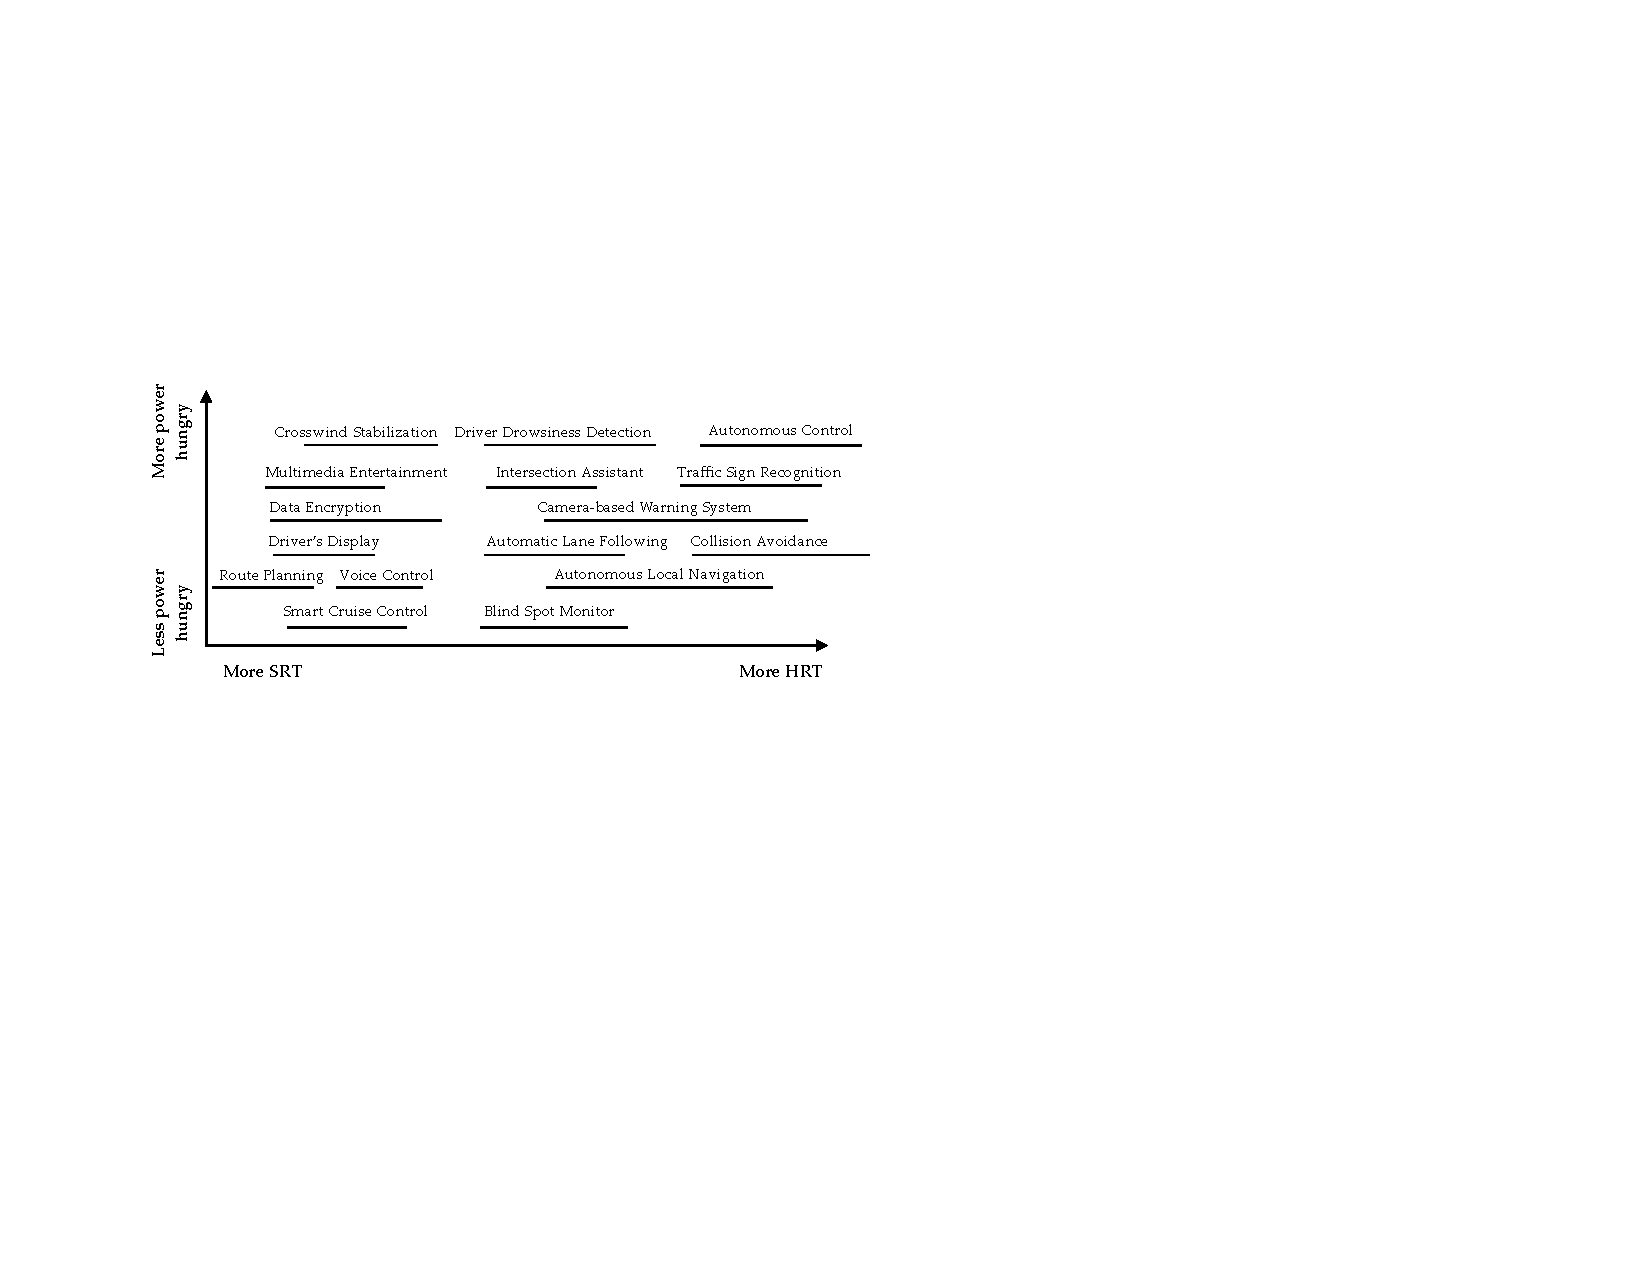
\includegraphics[width=4.6in]{images/automotive.pdf}
\vspace{-2mm}\caption{Spectrum of possible timing and energy requirements for a number of automotive workloads.}
\vspace{-4mm}
\label{fig:automotive}
\end{figure}

\paragraph{Automotive workloads.} 
\label{sec:automotiveworkload}

Heterogeneous computing platforms may be applied in a number of application domains where a wide range of timing and energy constraints are required. A particularly focused application domain we will investigate in this research is advanced driver-assisted automotive systems, where workloads with various timing and energy requirements are seen~\cite{elliott2011real}, as illustrated in Fig.~\ref{fig:automotive}.  
The automotive system represents an application domain where using heterogeneous computing platforms to achieve real-time performance and energy efficiency is particularly compelling. 
 In such systems, cores with different performance and energy characteristics can be allocated to workloads with different timing requirements. For example, more powerful cores can be used to process HRT workloads such as traffic sign recognition and collision avoidance; while less powerful but more energy efficient cores can be used to process SRT workloads such as voice control and route planning. Doing so may yield significantly less energy consumption compared to homogeneous platforms. % because less power-hungry workloads do not need to be processed by powerful cores, which results in necessarily high performance at the cost of energy loss.  Due to these reasons, heterogeneous computing platforms such as our targeted ARM's big.LITTLE are expected to see widespread adoption in automotive systems~\cite{armvehicle, armvehicle1, armvehicle2, armvehicle3}. 


\paragraph{Real-time OS.} The OS platform in this project will be an open-source real-time Linux extension called LITMUS$^{\textrm{RT}}$ \cite{LITMUS}. The PI was involved in developing this testbed~\cite{elliott1minimizing, Liudissertation}. The main purpose of LITMUS$^{\textrm{RT}}$ is to provide a useful experimental platform for applied real-time systems research. Currently LITMUS$^{\textrm{RT}}$ extends Linux by implementing a set of common scheduling algorithms as plug-in components. Numerous  publications \cite{elliott1minimizing, elliott1minimizing, Liudissertation, BBBdissertation, clustered, calandrino2008cache, johndissertation} have shown LITMUS$^{\textrm{RT}}$ to be a very valuable testbed for experimentally evaluating real-time scheduling algorithms by considering real system overheads. 
 Since big.LITTLE supports Linux (after setting a scheduler patch to add native big.LITTLE schedulers) and LITMUS$^{\textrm{RT}}$ is developed as a patch to the Linux kernel, we can run LITMUS$^{\textrm{RT}}$ on big.LITTLE for evaluation purposes.


%*********************************************************************************%

\subsection{Related Work}
\label{sec:relatedwork}
\vspace{1mm} \noindent \textbf{Real-time scheduling in heterogeneous systems.} The real-time scheduling of sporadic task systems on a homogeneous multiprocessors has received an enormous amount of attention~\cite{andersson2003, baker2007, funk2005, Baruah2006a, chattopadhyay2011, baruah2005a, baruah2008, bertogna2011b, BC, baruah1996, goossens2003, baker2003, Cluster1, davis2011a, devi2005, baruah1996, baruah2007, G, Par}.  On a heterogeneous multiprocessor that contains processor cores with varying speeds, several works~\cite{raravi2014task, raravi2013assigning, niemeier2011partitioned} have been conducted, which showed that partitioned scheduling-based approaches are able to yield HRT and SRT schedulability tests with various degrees of capacity loss. In a recent work~\cite{Tong14a}, PI Liu's research group  developed the first optimality result for this problem, which presents a global scheduling algorithm and its associated schedulability test that guarantees SRT correctness with no capacity loss. Another recent work~\cite{Chwa15} developed a new global scheduling algorithm and the associated schedulability test that guarantees HRT correctness with no capacity loss. 

\vspace{1mm} \noindent \textbf{Exploring timing-energy tradeoffs in heterogeneous systems.} For systems without timing requirements, a number of approaches have been proposed to explore the performance-energy tradeoffs (e.g., throughput versus energy)~\cite{muthukaruppan2014price, chen2014adaptive, muck2015run, sarma2015smartbalance, lin2014energy, tan2015approximation, elewi2014energy, annamalai2014reducing, yavits2014effect, beaumont2014analysis, gutierrez2014evaluating}. DVFS and dynamic power management policies have been used in such work to reduce energy consumption. %For the specific big.LITTLE platform, \cite{kim2015fair} proposed a new fair scheduler which is aware of the asymmetric platform and implemented in Linux on top of the big.LITTLE scheduler. In \cite{muthukaruppan2014price}, a price theory-based dynamic power management framework is designed to save energy on ARM's big.LITTLE.\cite{kim2014utilization} proposed utilization-aware load balancing mechanism target for energy efficiency of big.LITTLE processor. \cite{pathania2015power} developed an performance-aware Governor for mobile games to reduce energy consumption by leveraging power management tools such as DVFS.
 For systems with timing requirements, a couple of recent works~\cite{liuenergy, colin2014energy} have been conducted exploring the timing-energy tradeoffs in a heterogeneous computing system.  Besides yielding rather pessimistic schedulability tests (possibly due to the mere consideration of partitioned scheduling), these works apply a similar design philosophy as those designed for homogeneous platforms, where only timing-related concerns are considered when making scheduling decisions. Energy saving techniques such as DVFS are applied afterwards to the maximum degree to save energy while not causing timing violations. As will be discussed next in Section~\ref{sec:step1Motivation}, we believe that fundamental energy efficiency due to using a heterogeneous platform can only be achieved if  a scheduler considers the \textit{heterogeneous energy characteristics of tasks exhibited on different processors} when making scheduling decisions at the beginning.

%\paragraph{Schedulers native to big.LITTLE.} Clustered switching, in-kernel switcher, and global task scheduling are the three open-source scheduling modules native to the big.LITTLE architecture. Clustered switching is a simple implementation, arranging the processor into identically sized clusters of ``big'' or ``LITTLE'' cores. The OS scheduler can only see one cluster at a time and decides the specific cluster to execute a task. The in-kernel switcher pairs one big core with a LITTLE core. Each pair operates as one virtual core and only one real core is (fully) powered up and running at a time. For the pair in operation, one core is executing tasks while the other core is inactivated.   The most powerful native scheduler of big.LITTLE is global task scheduling, which enables the use of all physical cores at the same time. Computation-intensive tasks can be allocated to big cores while tasks with less resource-demanding requirements can be simultaneously allocated to little cores for energy efficiency purposes. The software are available on the Linaro git tree \cite{https://git.linaro.org/arm/big.LITTLE/switcher.git} as a patch set to the Linux kernel. 

\paragraph{DVFS approach overview.} DVFS has been proven to be an effective technique that reduces energy consumption through dynamically adjusting the supply voltage and operating frequency of processors. DVFS has also been widely studied in real-time embedded systems (see \cite{bhatti2011energy} for a detailed survey on this topic). DVFS-based real-time scheduling algorithms can be generally divided into three categories: (\textit{i}) \textit{static} DVFS, where DVFS are statically applied offline after all scheduling decisions (based on tasks' worst-case execution times) are made such that the frequency on every processor is minimized while still being able to guarantee timing correctness, (\textit{ii}) \textit{dynamic intra-task} DVFS, where variations (often called slack) in jobs' actual execution time and their pre-defined worst-case execution times are exploited. Slacks are dynamically reallocated inside the same task to further lower the frequency at runtime, and (\textit{iii}) \textit{dynamic inter-task} DVFS, which is similar to the dynamic intra-task DVFS approach but redistributes dynamic slack among other ready tasks. We will explore all these three DVFS approaches in our solution space.





%*********************************************************************************%
%*********************************************************************************%

\section{Detailed Research Plan}
\label{sec:researchplan}
\input{researchplan.tex}

%*********************************************************************************%

\subsection{Step 1: Identifying Energy-Efficient Configurations that Guarantee Timing}
\label{sec:step1}
We plan to develop fundamentally energy-efficient real-time scheduling algorithms and the associated schedulability tests that can be applied on heterogeneous platforms. Before describing our proposed approach, we first argue that the existing schedulers that are designed to guarantee timing correctness while minimizing energy consumption on a heterogeneous platform may actually be energy-inefficient.

\subsubsection{Motivation: Why Existing Energy-Efficient Real-Time Schedulers may be \sloppy{Energy-Inefficient}?} \label{sec:step1Motivation}

%The breadth of applications that can benefit from the usage of heterogeneous multiple processors includes many in which real-time constraints exist. In contrast to throughput-oriented applications, those with real-time constraints require predictable resource allocation methods that enable timing constraints to be validated. Energy-Aware Scheduling  issues arise when different resource allocation methods can be applied to schedule tasks on different processors while the applications' real-time requirements are satisfied.

Existing energy-efficient real-time schedulers on heterogeneous platforms (e.g., \cite{liuenergy, colin2014energy}) apply a similar design philosophy as those designed for homogeneous platforms. That is, tasks are first prioritized and scheduled to different processors according to their timing parameters to guarantee timing, then energy saving techniques such as DVFS are applied on a best effort basis to save energy while not causing timing violations. While it is generally more energy-efficient to use heterogeneous multiple processors instead of identical ones, we argue that fundamental energy efficiency due to using a heterogeneous platform can only be achieved if  a scheduler considers the \textit{heterogeneous energy characteristics of tasks exhibited on different processors} when performing task prioritization and processor selection, which are the two core operations of scheduling. The following example further illustrates this claim.

%\begin{figure}[H]
%\centerline{
%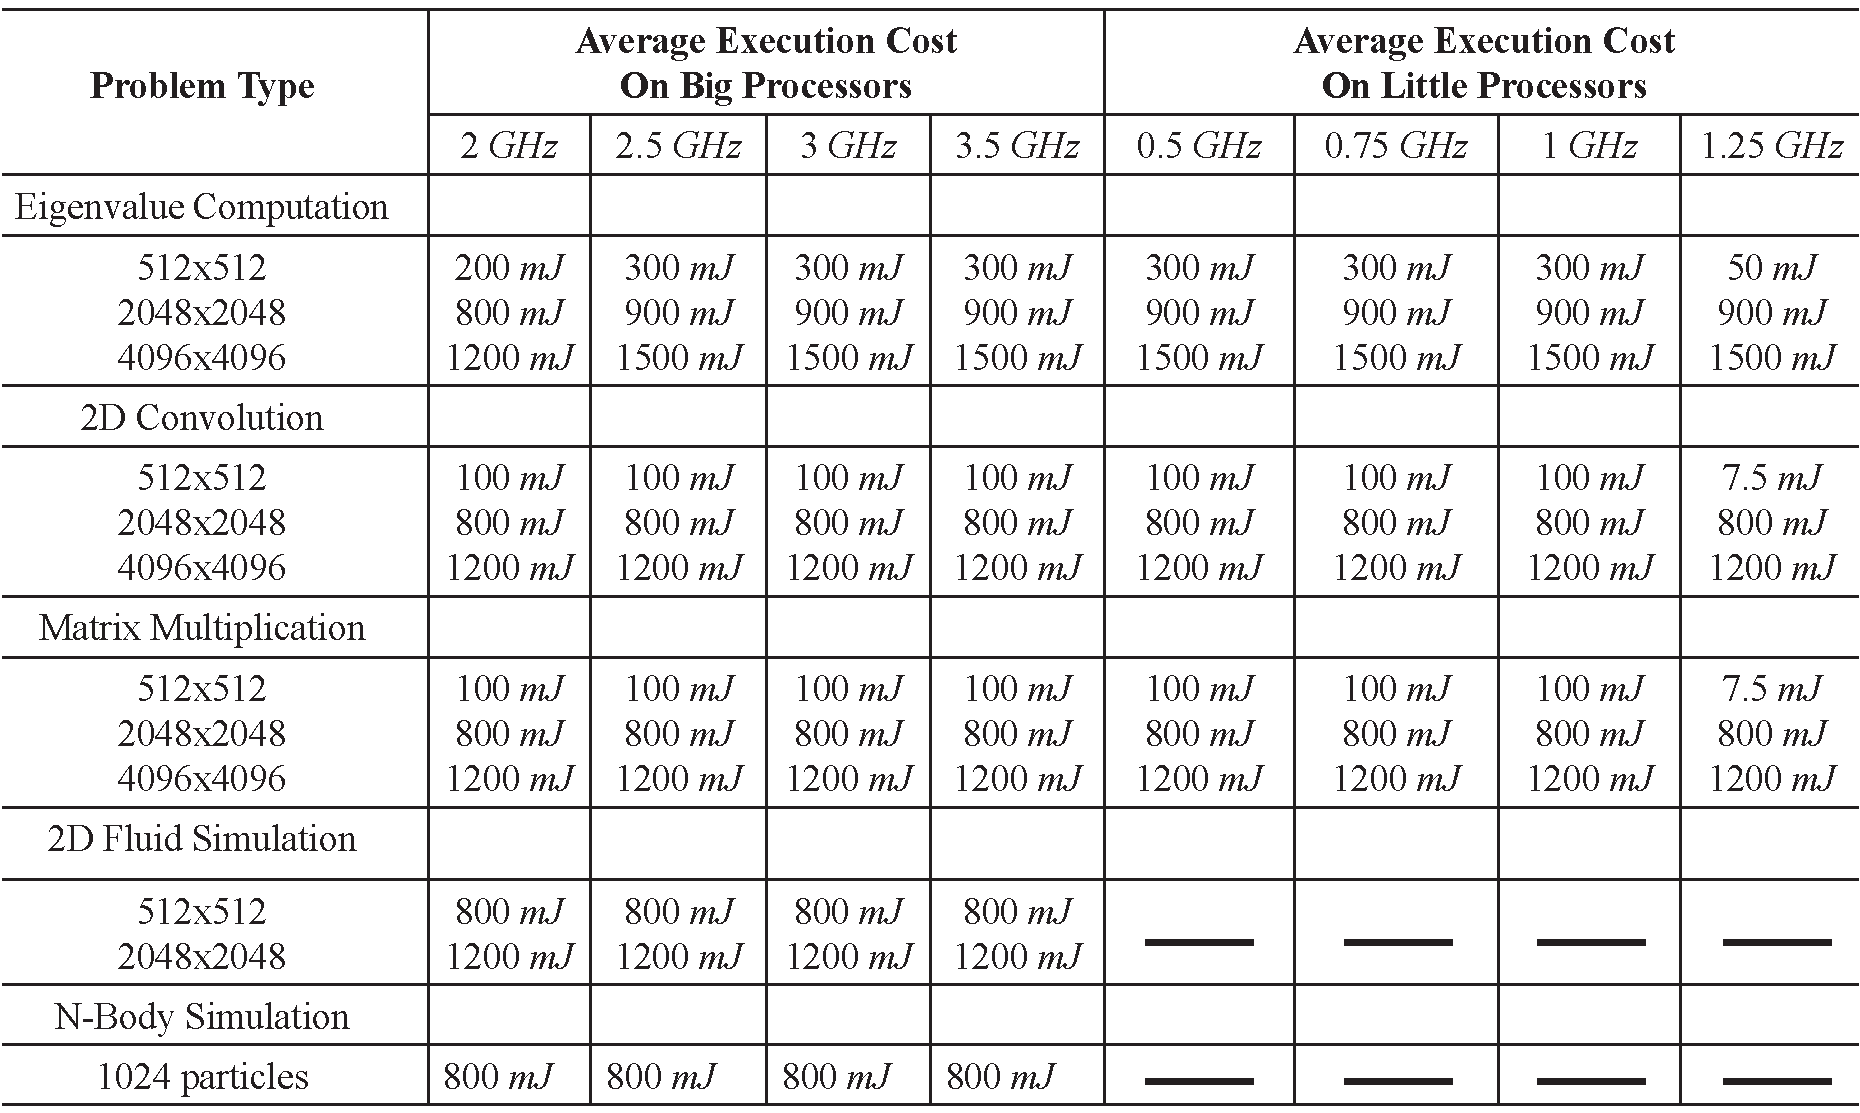
\includegraphics[width=0.65\columnwidth]{images/execution_cost.pdf}
%} \caption{Observed big.LITTLE execution cost under different frequencies.}
%\label{table:herogeneity}
%\end{figure}



 %Figure~\ref{table:herogeneity} summarizes the data we collected for the required energy to execute a job instance on different processors with different frequency settings on an ARM's big.LITTLE platform. 
 
 %As discussed earlier in Section~\ref{sec:hardware}, a key observation seen in Table~\ref{?} is that for certain workloads, the energy consumed on ``big'' processors with the lowest frequency is actually much larger than the energy consumed on ``LITTLE'' processors with the highest frequency. This indicates that if a task is first scheduled on a ``big'' processor to achieve the best  timing performance and then executed with a lowed frequency to save energy (i.e., the current practice), the resulting energy consumption may ironically be much larger than scheduling the task on a ``LITTLE'' processor according to its heterogeneous energy characteristics.  However, this observation does not simply suggest that all workloads shall be first scheduled to ``little'' processors to be energy efficient because (\textit{i}) doing so may cause timing violations due to the overloaded ``LITTLE'' processors, and (\textit{ii}) there also exist tasks whose heterogeneity in terms of the energy characteristics on different processors is rather small. Thus, we argue that the computing capacity provided by different processors to execute a particular task is required to be properly selected to save energy as the heterogeneity of processors arises, which can be further motivated by the following example.

%We illustrate this point by considering the generalized scheduling problem on big.LITTLE heterogeneous multiprocessor platforms, which we now define. Let $J = (r, c^{big}, c^{LITTLE}, d)$ denote a real-time job arriving at time $r$ and needing to execute for $c^{big}$ time units on ``big'' processors or $c^{LITTLE}$ time units on ``LITTLE'' processors by a deadline at time $d$.

%\textbf{The generalized heterogeneous multiprocessor scheduling problem}: Given a real-time instance $I = {J_1, J_2, . . . , J_n}$, and a specific heterogeneous multiprocessor platform~(e.g.~big.LITTLE), determine the smallest $E_{sum}$ such that instance $I$ is feasible upon a platform of total energy consumption $E_{sum}$, in which no job violates its HRT or SRT timing requirement.


\begin{wrapfigure}{r}{0.55\textwidth}
\vspace{-4mm}
\centerline{
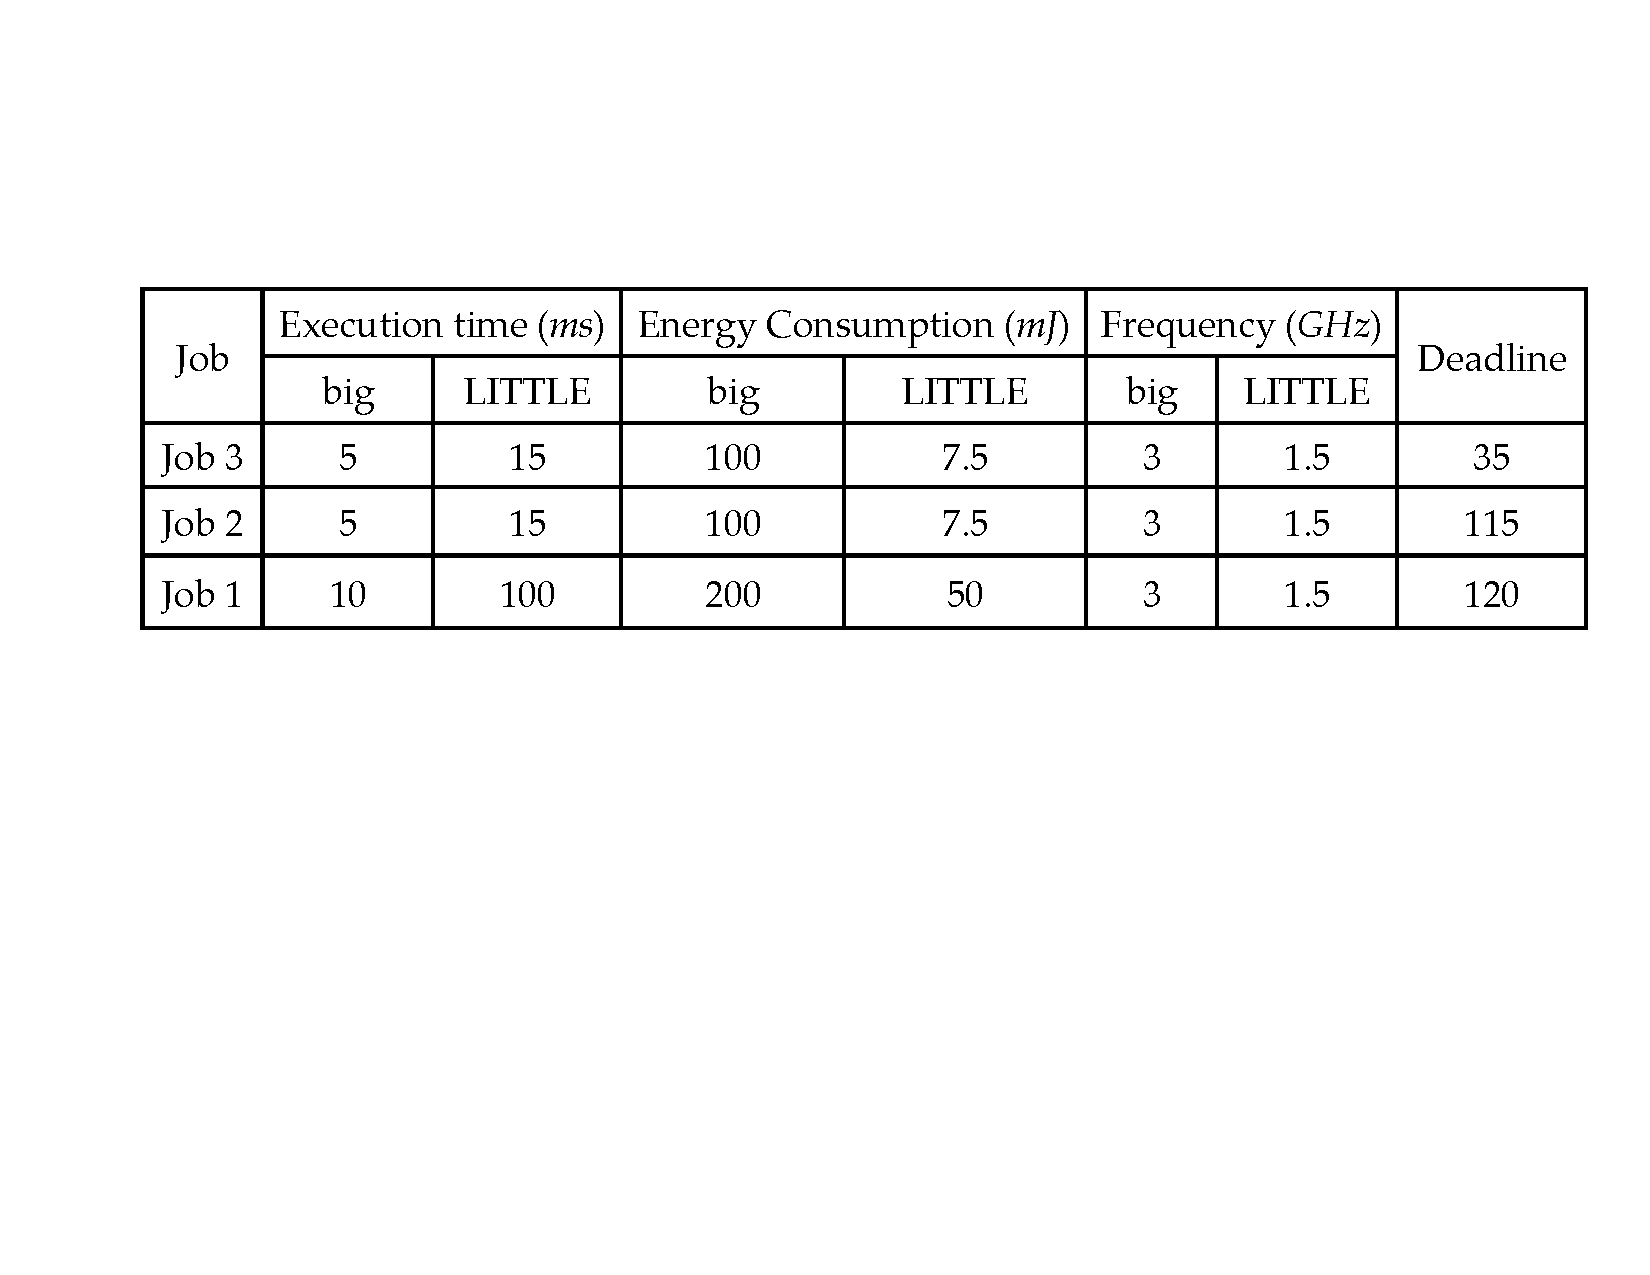
\includegraphics[width=0.55\columnwidth]{images/example_table.pdf}
} \caption{\small An example job set run on  big.LITTLE.}\vspace{-4mm}
\label{fig:big.little}
\end{wrapfigure} \normalsize

\paragraph{Example.}
An example job set is comprised of the following three jobs:
\begin{itemize}
\item $J_1$ = (0, 10, 100, 120); $J_2$ = (0, 5, 15, 115); $J_3$ = (0, 5, 15, 35),
\end{itemize}
 where $J = (r, c^{big}, c^{LITTLE}, d)$ denotes a real-time job arriving at time $r$ and needing to execute for $c^{big}$ time units on ``big'' processors or $c^{LITTLE}$ time units on ``LITTLE'' processors by a deadline at time $d$. 
 The platform associated parameters are shown in Figure~\ref{fig:big.little}. Suppose that we wish to schedule this instance on a big.LITTLE platform in which processor speeds will remain static during run-time (note that we can apply  DVFS on different processors later to further save energy). We consider three different schedulers. The first scheduler is the classical real-time scheduler GEDF, with the resulting schedule shown in Figure~\ref{fig:edf}. Under GEDF, the job with the earliest deadline will be scheduled on an earliest available processor. The GEDF schedule completes all three jobs by their deadlines, but yielding a total energy consumption of 307.5 mJ. Figure~\ref{fig:workconserving} shows a modified work-conserving schedule where job prioritization and core selection are made by considering both timing- and energy-related parameters. Since $J_1$ exhibits the highest degree of heterogeneity in terms of the difference between the energy consumed on two types of processors, we assign the highest priority to $J_1$, the second highest priority to $J_3$, and the lowest priority to $J_2$ (which has the longest deadline). Doing so allows $J_1$ to be allocated to the ``LITTLE'' processor and the resulting energy consumption can be reduced to 250 mJ. Notice that $J_2$ is assigned to the ``big'' processor since this processor idles first at time 5. Under the third scheduler, as shown in Fig.~\ref{fig:optimal}, the energy consumption can be further reduced to 157.5 mJ (which is optimal for this example). This is by employing a non-work-conserving scheduler, which enforces $J_2$ to wait to be scheduled on its favorite processor in terms of energy consumption, even if its unfavorable ``big'' processor becomes idle at time 5.


 
 \begin{figure*}
\centering
\subfloat[]{\label{fig:edf}
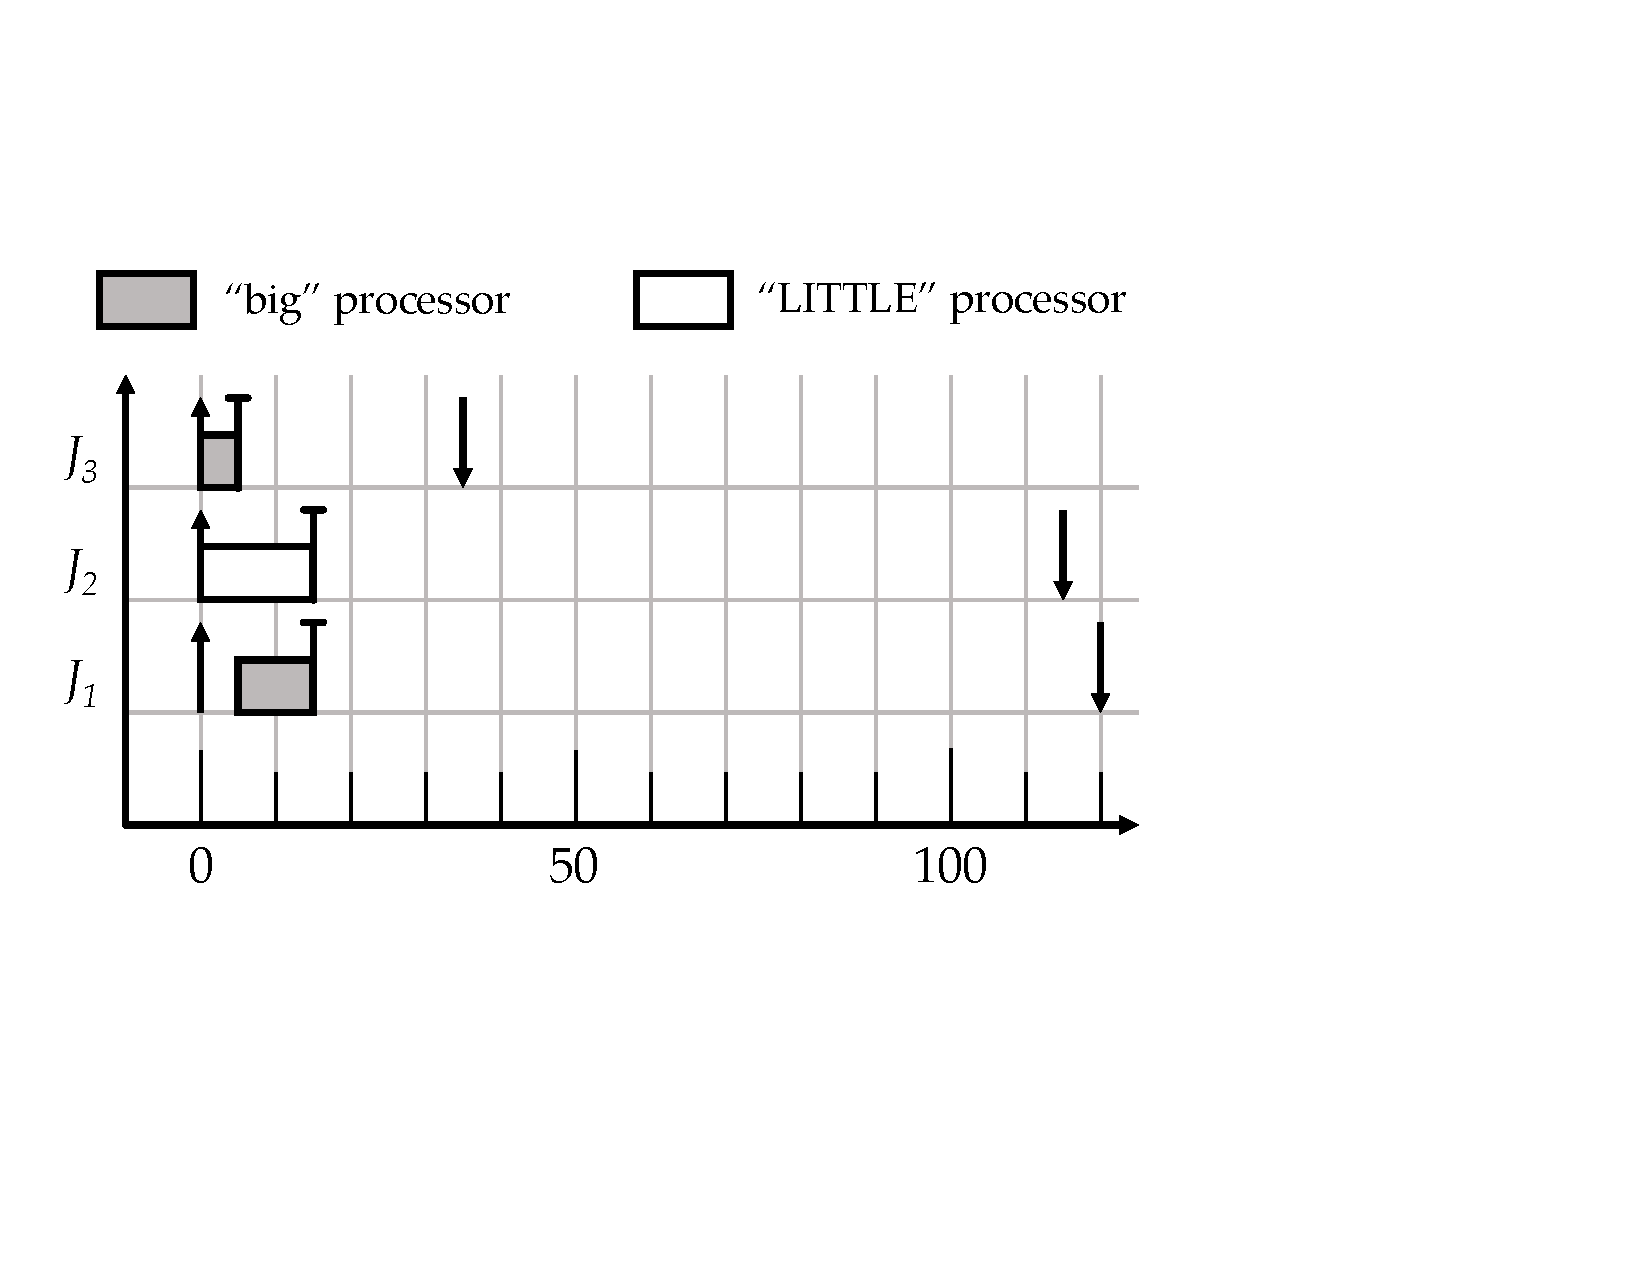
\includegraphics[width=0.32\columnwidth]{images/example_1.pdf}}
\subfloat[]{\label{fig:workconserving}
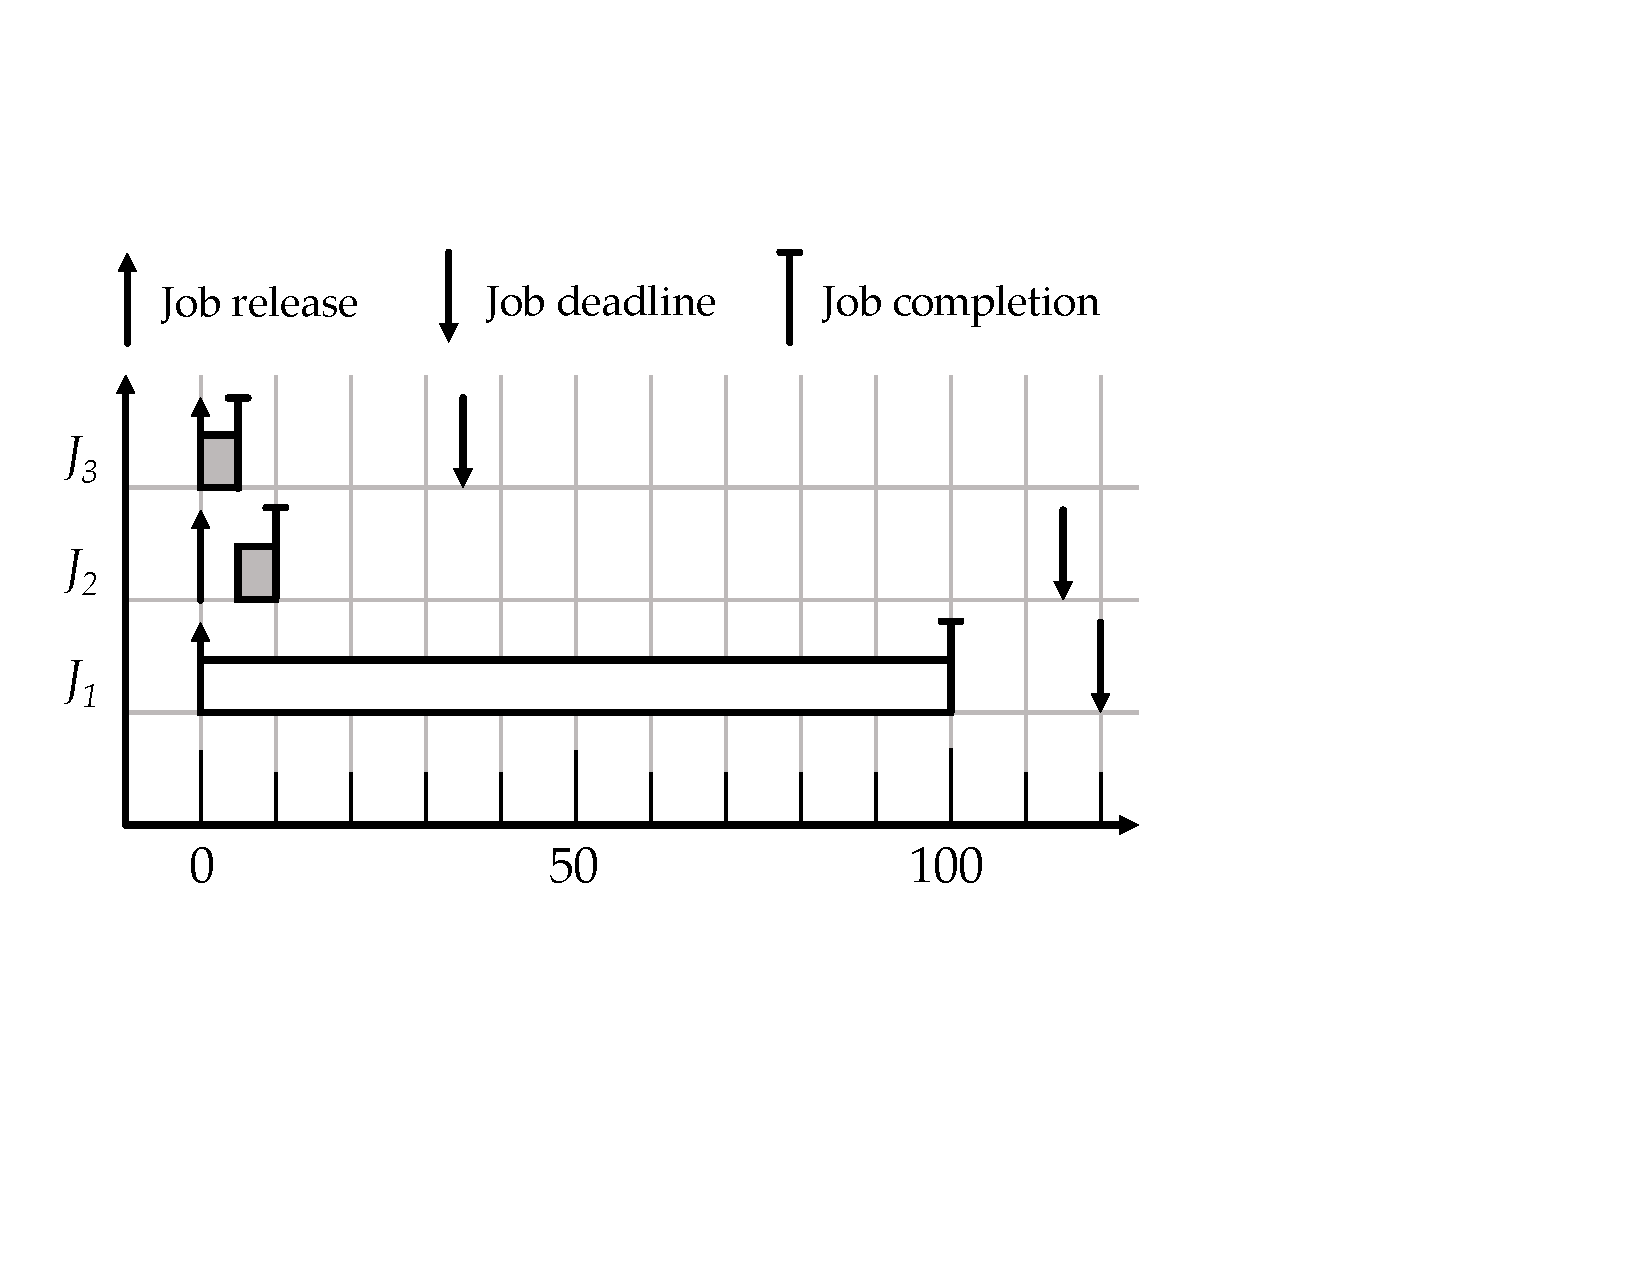
\includegraphics[width=0.32\columnwidth]{images/example_2.pdf}}
\subfloat[]{\label{fig:optimal}
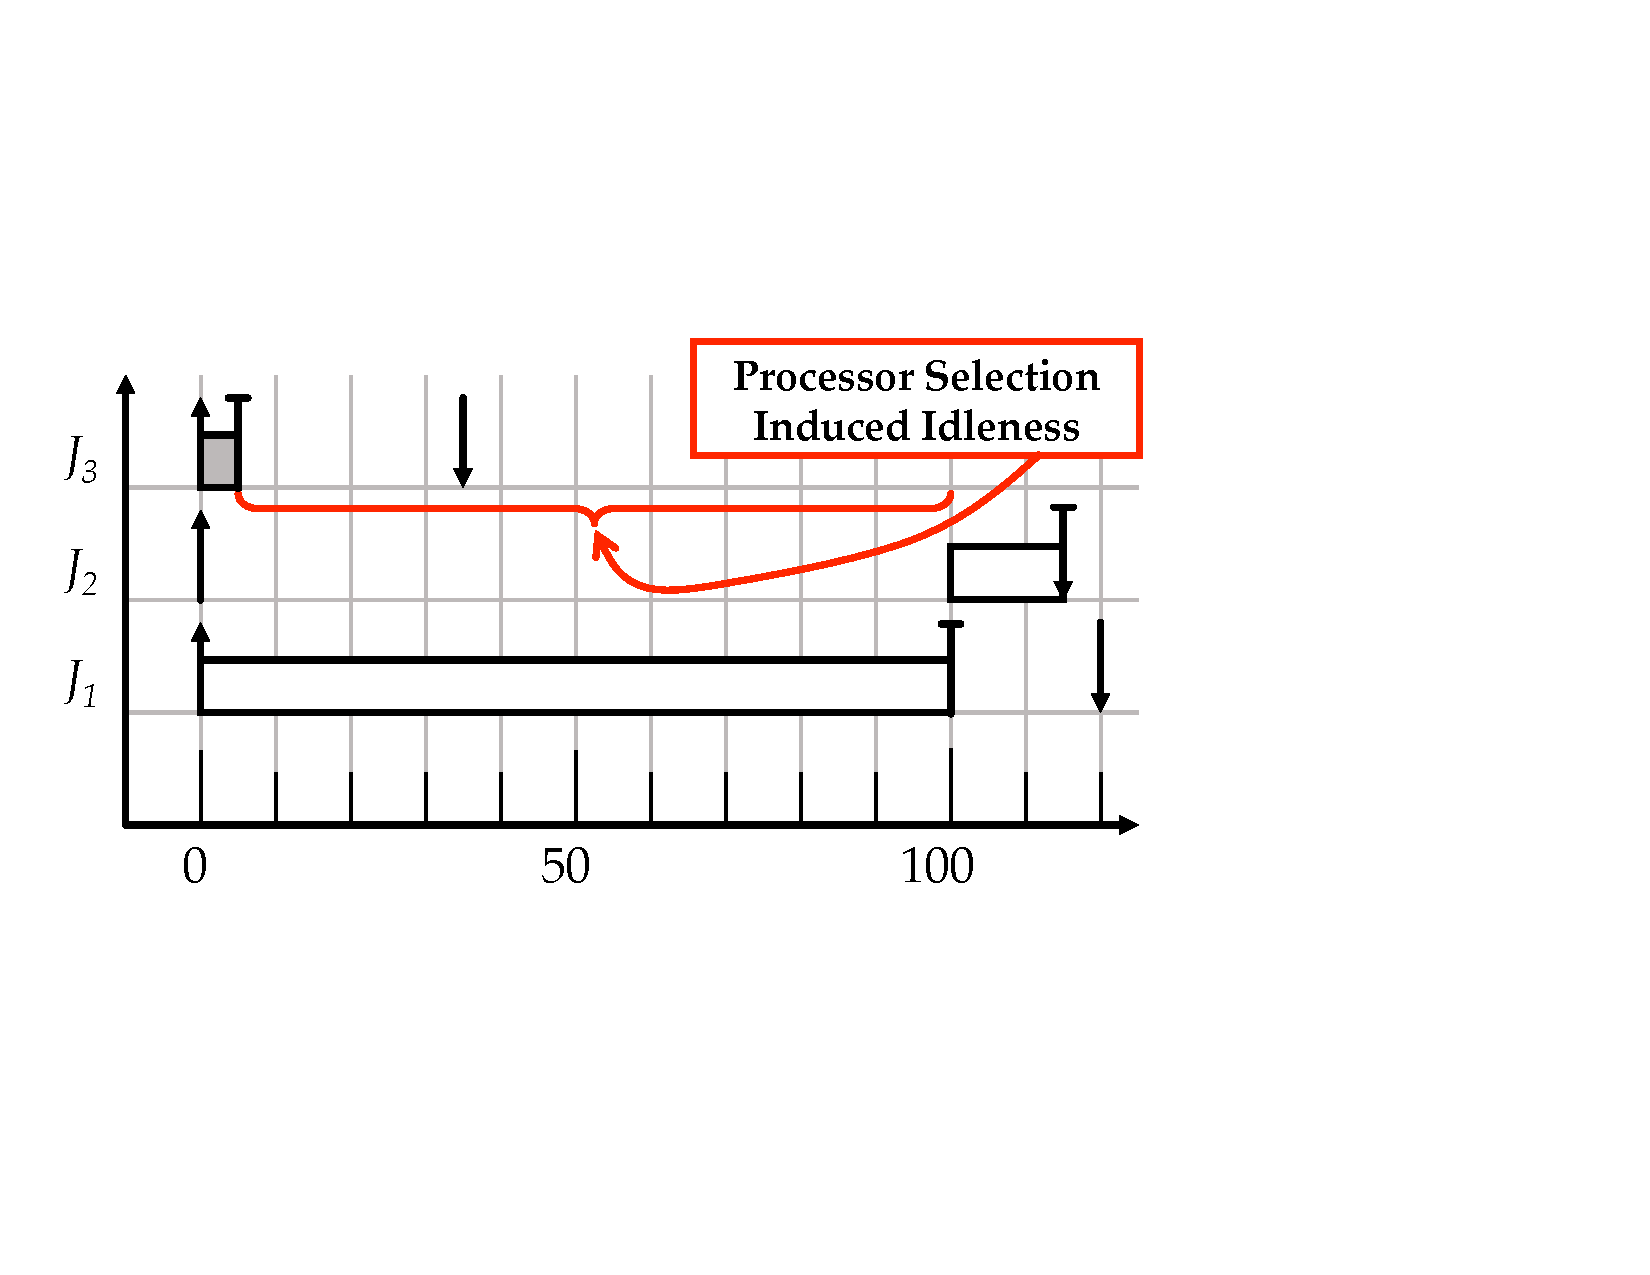
\includegraphics[width=0.32\columnwidth]{images/example_3.pdf}}
\vspace{-2mm}
\caption{\small (a) G-EDF yields $307.5~mJ$; (b) A work-conserving energy-aware scheme yields $250~mJ$; (c) A non-work-conserving energy-aware scheme yields $157.5~mJ$.}\normalsize
\vspace{-2mm}
\end{figure*}

The above example highlights the motivation behind our design of energy-efficient real-time schedulers on heterogeneous platforms, that is, fundamental energy efficiency on heterogeneous platforms can be achieved when a scheduler determines both job prioritization and processor selection by considering tasks' heterogeneous energy characteristics on different processors as first-class citizen.
% Moreover, as this example shows, there is a non-trivial relationship between the minimum amount of required energy by a real-time instance, and the scheduling method that is feasible to satisfy timing requirements. For simple workloads comprised entirely of a fixed collection of independent jobs (as in the the example above), it may be possible to present this solution space as a collection of simple constraints, and identify optimal solutions using standard optimization techniques. However, the problem becomes considerably more difficult if the instance to be scheduled is represented more succinctly than by enumerating all jobs (e.g., as sporadic tasks). Solving this problem is an essential prerequisite to obtaining optimal or near-optimal energy-efficient implementations of embedded real-time systems. Consequently, one of our major goals is to obtain general solution techniques for solving the problem of real-time task scheduling on a heterogeneous platform that yields the minimum energy consumption.


\paragraph{Energy-oriented task prioritization and processor selection schemes.} We propose to investigate a number of potential task prioritization and processor selection schemes that make decisions by considering tasks' heterogeneous energy characteristics. Note that any of these schemes will be viewed as a core component of each different scheduling methodology (e.g., partitioned, clustered, or global scheduling, as will be discussed  in Section~\ref{sec:step1Config}). We will investigate the following two categories of such schemes:

\begin{itemize}\itemsep 0pt \parskip 0pt
\item[1.] \textbf{Energy-efficient schemes (EES):} We first apply classical real-time task prioritization schemes (e.g., EDF or rate monotonic), and then schedule each task to the processor that yields the minimum energy consumption while guaranteeing timing correctness. The tradeoff herein is that applying classical timing-oriented task prioritization may yield tighter schedulability analysis; while applying energy-oriented processor selection may yield better energy efficiency.
\item[2.] \textbf{Energy-aggressive schemes (EAS):} For more aggressive energy savings, we will apply a set of energy-oriented task prioritization rules, and then schedule each task to the processor that yields the minimum energy consumption while guaranteeing timing correctness. We propose to consider the following energy-oriented task prioritization rules: (\textit{i}) largest-energy-heterogeneity-ratio-first: tasks with the higher energy heterogeneity ratio will be assigned higher priorities, where a task's energy heterogeneity ratio is defined to be  the energy consumed for running it on a ``big'' processor divided by the energy consumed for running it on a ``LITTLE'' processor. The intuition is that more energy would be wasted if a task with a higher energy heterogeneity ratio is scheduled to an unfavorite type of processor in terms of energy. (\textit{ii}) largest-energy-difference-first: tasks with larger energy difference values will be assigned higher priorities, where a task's energy difference is defined to be the difference between the energy consumed for running it on a ``big'' processor and a ``LITTLE'' processor. (\textit{iii}) largest-energy-timing-ratio-first: tasks with higher energy-timing ratio will be assigned higher priorities, where a task's energy-timing ratio is defined to be the minimum value between the energy consumed for running it on either a ``big'' or a ``LITTLE'' processor divided by the task's relative deadline.
\end{itemize}

We will discuss next how to incorporate the above energy-oriented task prioritization and processor selection schemes into the vast solution space.

\subsubsection{Identifying Energy-Efficient Configurations that Guarantee Timing}
\label{sec:step1Config}

We plan to devise energy-efficient real-time scheduling methods and the corresponding HRT and SRT schedulability tests that can be applied on heterogeneous computing platforms. These tests will account for runtime system overhead incurred under different methods.

The basic resource allocation methods that we believe will be the most fruitful is to apply DVFS combined with energy-oriented scheduling (i.e., EES and EAS) to reduce energy consumption. This is motivated by our experimental data showing that for many applications, scaling down the frequency yields considerably more energy saving than race-to-idle (as discussed in Section~\ref{sec:hardware}). The solution space for defining such resource allocation methods is vast. As noted earlier, processor capacity can be allocated on a partitioned, clustered, or global basis. Priorities can be assigned on a per-job (i.e., dynamic-priority scheduling such as EDF) or per-task (i.e., static-priority scheduling such as rate monotonic) basis. For each combination, the three DVFS methods (discussed in Section~\ref{sec:relatedwork}) can be applied.

\begin{wrapfigure}{R}{0.43\textwidth}
\vspace{-2mm}
\centerline{
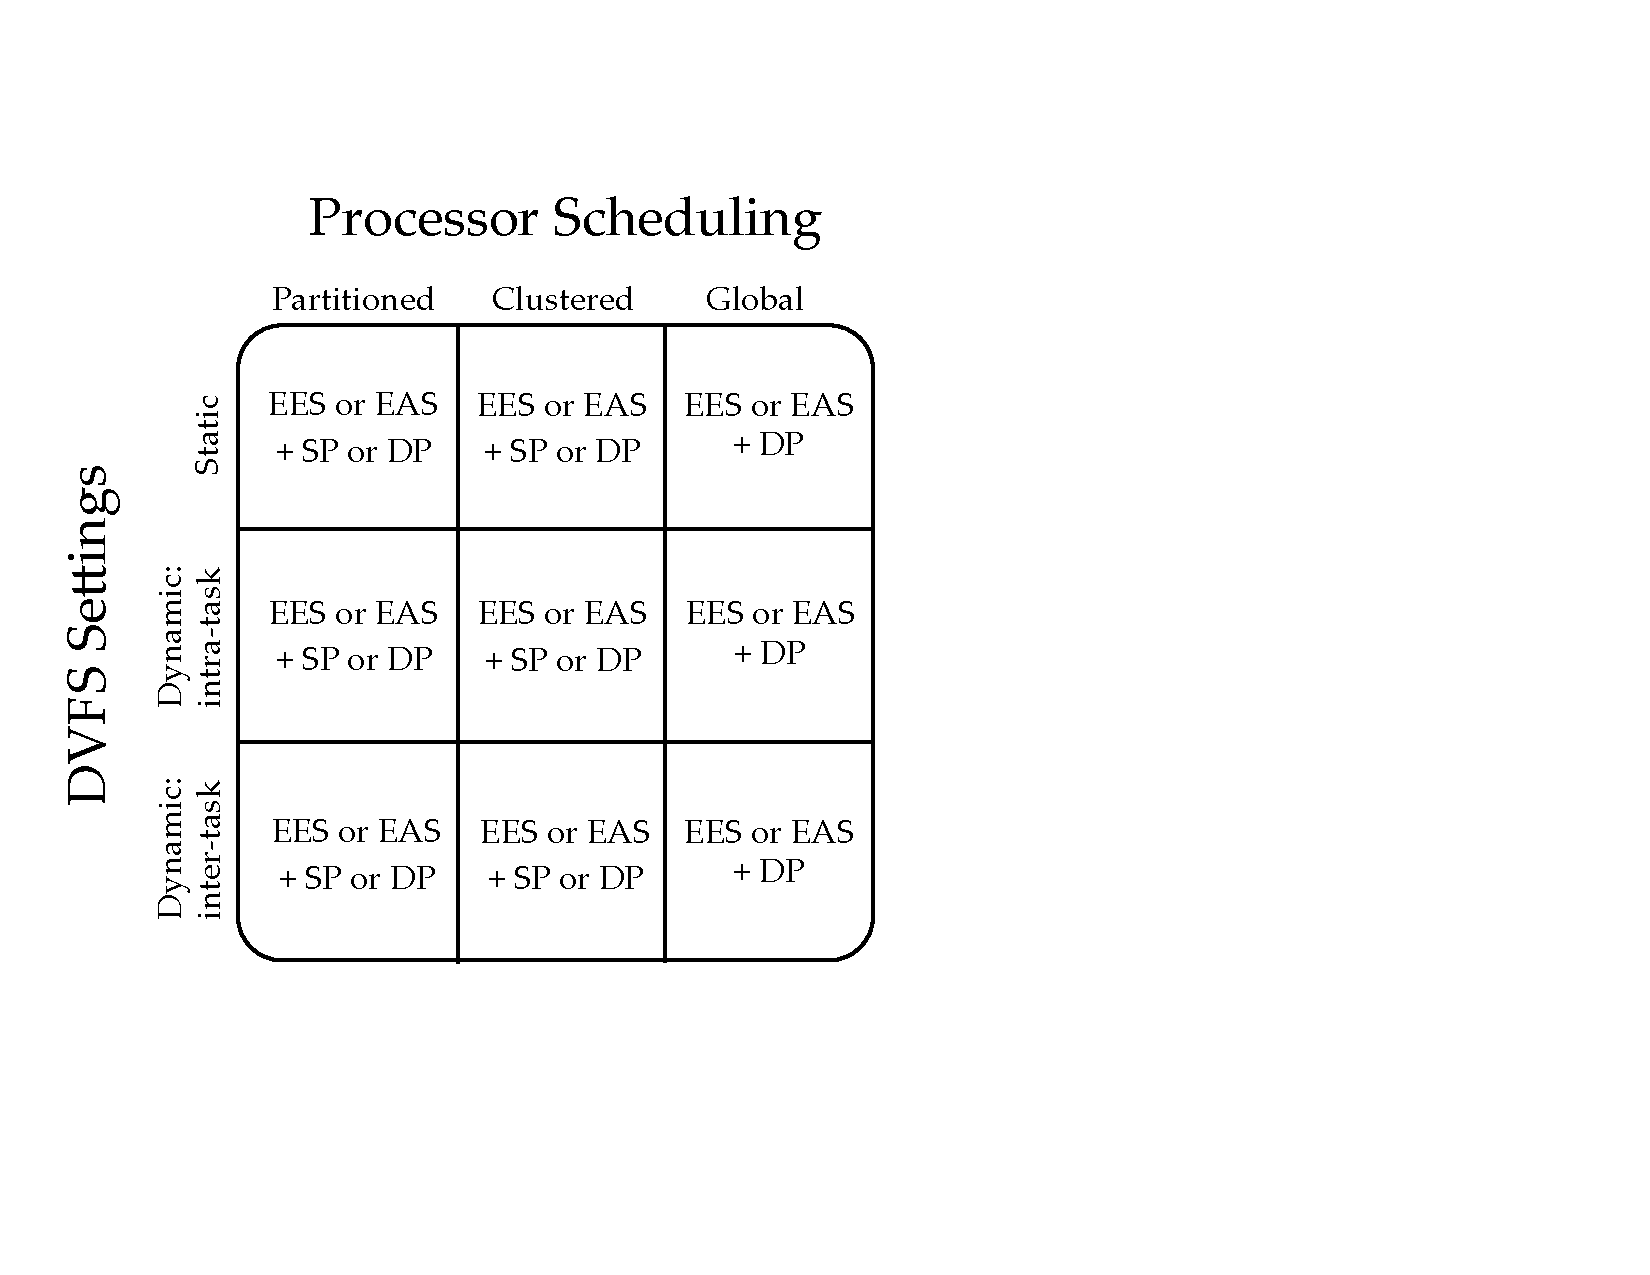
\includegraphics[width=0.42\textwidth]{images/configurations.pdf}
} \caption{\small Potential configurations.}\normalsize
\label{fig:configurations}
\end{wrapfigure}
 Although the solution space is large, our proposed energy-oriented EES and EAS can be generally applied to almost all settings. For example, when processors are globally managed, capacity can be allocated using dynamic-priority EES with processing frequency controlled by the static DVFS method.  This is because all the components included in each configuration are mostly independent. Each configuration contains four components: (processor allocation, task prioritization and core selection, priority assignment, DVFS), where each component has several settings, as illustrated in Figure~\ref{fig:configurations}. Note that the only configurations we do not intend to investigate are the combination of static-priority and global scheduling, as previous work~\cite{bastoni2010empirical} has shown that such approaches may cause significant capacity loss in multicore systems.
  Each configuration may have its benefits. For example, as noted earlier, partitioned approaches generally perform well in HRT domains, while global approaches typically perform better in SRT domains. 
 
 
\begin{comment}

\begin{wrapfigure}{R}{0.45\textwidth}
\vspace{-3mm}
\centerline{
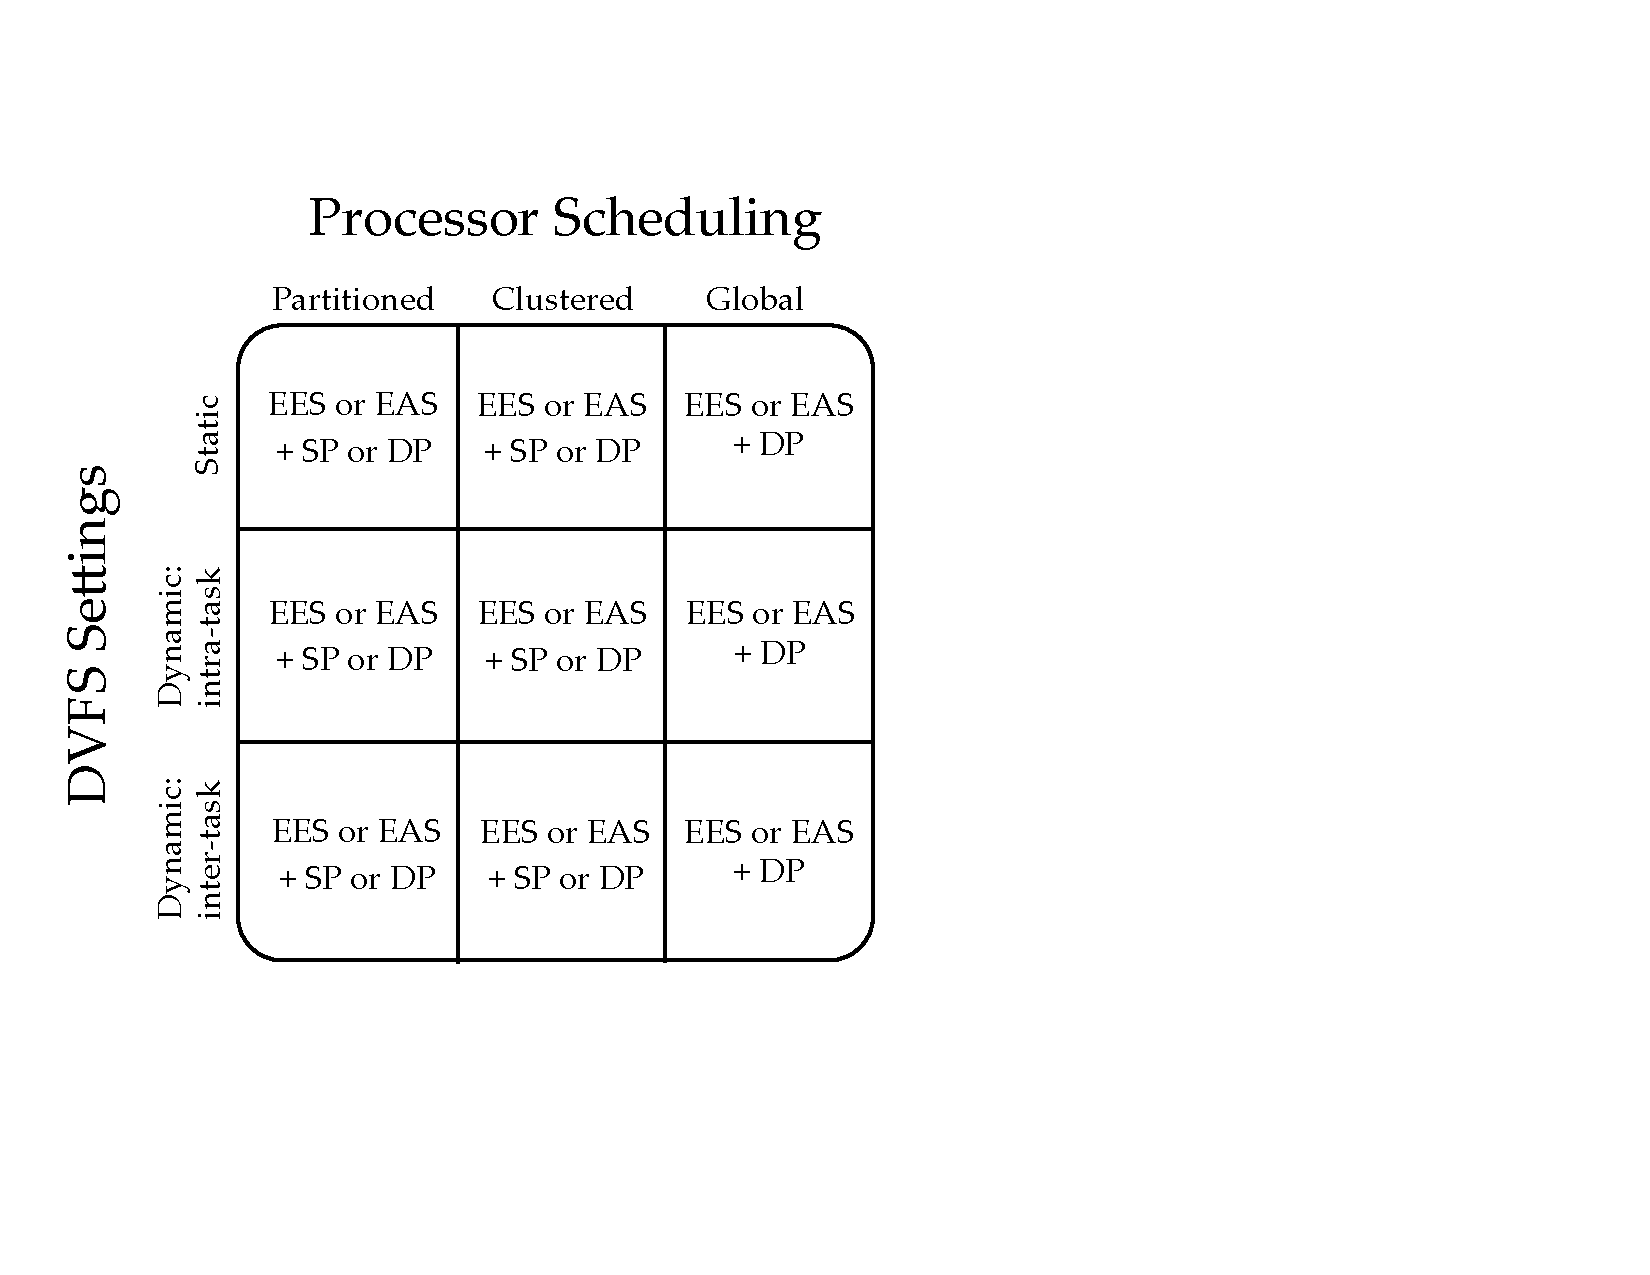
\includegraphics[width=0.42\textwidth]{images/configurations.pdf}
} \caption{\small Processor scheduling and DVFS settings under either fixed-priority (FP) or dynamic-priority (DP) EES and EAS scheduling schemes.}\normalsize
\label{fig:configurations}
\end{wrapfigure}

\end{comment}

 

While  Figure~\ref{fig:configurations} implies that there are 36 different configurations, each configuration can be even further specialized. For instance, a single ``big'' processor does not necessarily need to be bound to a single ``LITTLE'' processor under clustered scheduling. Instead, a single ``big'' processor could be clustered along with several ``LITTLE'' processors. However, this minor change yields new challenges when we assign tasks to processors, since the symmetric processor structure (i.e., one ``big'' and one ``LITTLE'' processor) now changes to an asymmetric one (i.e., one ``big'' and multiple ``LITTLE'' processors). This change forces the consideration of other alternatives. We have identified over twenty possible big/LITTLE scheduling/organizational combinations for dynamic-priority systems alone. The situation is similar for static-priority systems. Matters are further complicated by other factors. For example, HRT and SRT systems are subject to different schedulability analysis. Finally, to be practicably applicable, schedulability tests must be augmented to account for system overheads such as OS activities and cache-related preemption and migration costs. %For example, global approaches may be sound in theory but suffer in practice due to frequent job preemption and migrations. 
 The proper accounting of such overheads is extraordinarily tedious as we experienced in our previous work~\cite{Liudissertation, elliott1minimizing}. The major goal in Part 1 of this project is to sift through all of these analysis alternatives, devise the tightest schedulability analysis that is practicably possible for each alternative. The most energy-efficient ones among these alternatives will also be identified through implementation and extensive evaluation. % (as detailed in Sections~\ref{sec:implementation} and \ref{sec:evaluation}). 

%\paragraph{DVFS-oriented approaches.} While we believe that the above DVFS-based approaches will prove to be the most effective in improving energy efficiency, we are not wedded to this idea and will be open to other approaches. A particular idea we will explore is to develop DVFS-oriented approaches. The DVFS-based approaches seek to treat DVFS as an energy optimization approach (i.e., first identifying scheduling and then apply a specific DVFS approach). The DVFS-oriented approaches instead seek to improve energy efficiency from the opposite direction, where the most energy-efficient frequency choices for all processors will first be identified, under which a feasible timing-correct schedule can be derived. 

%The traditional task scheduling problem can be considered as a classic bin-packing problem that is NP-hard in the strong sense~\cite{coffman1978application}. When we apply DVFS, it becomes a bin-packing problem where bins have capacities that can be varied, because different frequencies yield different task execution times. Thus, identifying an optimal frequency selection method for task scheduling on a heterogeneous platform is clearly NP-hard in the strong sense. Thus, algorithms that approximate an optimal solution are often used in practice. A polynomialtime approximation scheme (PTAS) is a particularly appealing approximation approach that allows runtime performance to be traded for approximation accuracy.  Recent work has shown that a PTAS exists for real-time tasks scheduled on two types of processors under EDF (without applying DVFS)~\cite{baruah2011task}. We intend to develop frequency selection methods based on such existing solutions for correctly scheduling real-time tasks on heterogeneous platforms with minimum energy consumption.  At the very least, we will develop and experimentally analyze useful frequency selection heuristics for task scheduling algorithms. However, we prefer to obtain methods like PTASs for which provable approximation bounds can be obtained.




%*********************************************************************************%

\subsection{Step 2: ...}
\label{sec:step2}
In step 2, we will develop new algorithms and techniques that address
energy consumption for mixed critical real-time systems such as
automotive computing.  In both cases, we plan to leverage two key
insights about heterogeneous architectures like those presented in
Figure~\ref{tradeoffs}:
\begin{itemize}
\item Their energy efficiency increases as they slow down.
\item They have tremendous additional compute capacity that can only
  be used for short amounts of time.
\end{itemize}

Specifically, we will develop two techniques, each based off one of
these insights, and each providing a different capability:
\begin{itemize}
\item \textbf{Pace-to-sprint}: The goal of this technique is to reduce
  energy consumption for hard real-time workloads.  Where traditional
  techniques allocate for worst case and then idle if work is
  completed early (i.e., race-to-idle), pace-to-sprint will develop
  scheduling techniques to spend as much time as possible in slower,
  more energy-efficient states.
\item \textbf{Energy Guarantees}: The goal of this technique will be
  to guarantee energy consumption for mixed critical workloads; i.e.,
  workloads that contain jobs with both hard and soft real-time
  requirements.  In this work, we will use the additional,
  unsustainable compute capacity to process hard real-time tasks and
  ensure that their deadlines are respected (building off our work in
  step 1).  In addition, we will develop algorithms and interfaces for
  admitting additional soft real-time jobs that will only be scheduled
  if they do not violate energy constraints.  Thus, this technique
  will allow us to bound both timeliness and energy consumption,
  possibly at the cost of not executing some non-critical tasks.
\end{itemize}


\subsubsection{Pace-to-Sprint}
We will develop pace-to-sprint techniques to minimize energy
consumption.  The key insight here is that allocating for worst case
execution time...

Linear optimization?




\subsubsection{Energy Guarantees for Mixed Critical Workloads}
We will develop techniques to provide energy consumption guarantees
for systems with both hard and soft real-time requirements.

Take energy budget.  Divide into periods.  Determine average power per
scheduling period.

Hard real-time tasks scheduled using big cores.  When those complete,
determine remaining available power.  Run best-effort tasks in
configuration that meets available power requirement.


\subsubsection{Evaluation}

We will evaluate our techniques along two metrics: energy consumption
and schedulability.

Energy consumption of pace-to-sprint should be lower than existing
techniques, specific savings will depend on workload, but maybe a
factor of two better than race.

Schedulability of our guaranteed techniques should be higher than
current techniques.


%*********************************************************************************%

\subsection{Step 3: Implementation and Overhead-Conscious Schedulability Studies}
\label{sec:step3}
After conducting the research summarized in Sections~\ref{sec:step1} and \ref{sec:step2}, we will have a set of energy-efficient real-time scheduling methods on heterogeneous computing platforms. This section discusses our implementation plan and evaluation work needed to assess which methods are preferable from the perspectives of overhead-conscious schedulability, runtime response times, and energy consumption. 

\vspace{-2mm} \paragraph{Implementation plans.} We will implement our proposed resource allocation methods in real systems to evaluate their performance in practice. The OS platform will be LITMUS$^{\textrm{RT}}$~\cite{LITMUS}. As discussed earlier, our goal of using LITMUS$^{\textrm{RT}}$ is to have a useful experimental platform for evaluating overhead-conscious schedulability of our proposed scheduling methods. 
As discussed earlier, ARM's big.LITTLE supports Linux. The two open-source scheduling modules, i.e., kernel switcher and global task scheduling~\cite{armscheduler}, can be patched to the Linux kernel. Thus, we will patch LITMUS$^{\textrm{RT}}$ to the Linux kernel running on big.LITTLE. 
Each of our proposed methods  will be implemented in LITMUS$^{\textrm{RT}}$ as a plugin component. (This implementation method allows users to switch between different scheduling policies at runtime.)  %An interesting set of experiments would be to compare the timing and energy performance between our proposed methods and the native kernel switcher and global task scheduling methods on big.LITTLE. 
 To measure energy consumption, we will use the two currently available tools. The first tool is the ARM DS-5 Streamline tool set\cite{ARMDS5}, which is a performance analyzer that brings together system performance metrics, software tracing, statistical profiling and power measurement through user interface. The second tool is to the INA231 Current/Power monitor chip produced by TI \cite{israelssonenergy, INA231, hahnel2014heterogeneity}. The power data is obtained through measuring both the shunt voltage drops and bus supply voltage. The ODROID-XU3 board~\cite{ODROIDXU} powered by ARM big.LITTLE technology already integrates four INA231 monitors that can measure the energy data of the ``big'' cluster, ``LITTLE'' cluster, GPU, and memory \cite{hahnel2014heterogeneity}. We currently have a cluster of 12 ODROID-XU3s in our research lab for implementation and evaluation purposes.  

We also intend to consider heterogeneous multicore platforms from other manufactures as well as those adopting similar heterogeneous system architectures. For instance, we plan to consider another  two heterogeneous multicore architectures that are similar to big.LITTLE, i.e., NVIDIA's Tegra 3 SoC~\cite{KalEI} and Freescale's Vybrid SoC~\cite{VybridController}. Tegra 3 adopts a variable symmetric multiprocessing technology, which aims to minimize the active standby state power consumption but still deliver required performance. Tegra 3 includes an ARM's quard-core Cortex A9 processor for high performance and one companion CPU which is energy-efficient but delivers relatively low performance. The platform can save energy by scheduling less resource-demanding task to the companion CPU. Compared to big.LITTLE, Tegra 3 may yield a milder solution for energy saving and a smaller range for energy-performance tradeoff. Freescale's Vybrid SoC also applied asymmetric architecture, but for the purpose of separating user-interface workloads and real-time workloads. The platform consists of one ARM Cortex-A5 processor running Linux and one ARM Cortex-M4 core running real-time operating systems like freescale's MQX. A multicore communication protocol is designed to coordinate the interactions between the two processors. Compared to big.LITTLE architecture, the Vybrid architecture mainly deals with the conflicts between real-time and non-real-time workloads other than the tradeoff between energy and performance.

\vspace{-2mm} \paragraph{Overhead-conscious schedulability and energy studies.} A research focus herein is to sift through all resource allocation options identified in Sections~\ref{sec:step1} and \ref{sec:step2} through evaluating the performance with respect to schedulability and energy efficiency when practical scheduler-incurred overheads are considered. The overhead-conscious evaluation is important as a theoretically-sound scheduler may not perform well in practice. For example, although global scheduling approaches generally yield better theoretical schedulability tests with less capacity loss than partitioned approaches, they may perform worse than partitioned approaches due to the more frequent task preemption and migrations.

To evaluate the performance with respect to overhead-conscious schedulability and energy efficiency, we will follow a mature experimental process applied in many previous work \cite{BBBdissertation, clustered, bastoni2010, calandrino2007, johndissertation}. Actual system overheads will be gathered and considered in this process. Scheduling actions may incur various types of overheads, including costs due to scheduling decisions, context switch operations, task queue management, interrupt servicing, and preemption and migration. By implementing our proposed energy efficient heterogeneity-aware scheduling algorithms in LITMUS$^{\textrm{RT}}$, we will be able to gather these overheads under different approaches using millions of randomly generated task systems and benchmarks.  After collecting overheads, we will factor them into task parameters and check the schedulability of all generated task systems. The outcome of this experimental process is a collection of schedulability graphs showing how different scheduling approaches perform and compare in light of real system overheads. Besides schedulability, energy consumption, response time bounds (analytically derived under our derived schedulability tests) and run-time response times are also important. We will also evaluate the proposed methods in terms of energy consumption, and maximum and average runtime response times.  

%*********************************************************************************%

\subsection{Step 4: Conduct Case Studies}
\label{sec:step4}
In order to further access whether our proposed methods can be applied in practical systems, we intend to conduct case-study evaluations using actual workloads from an advanced automotive system. Due to space constraints, we describe one proposed case study in (some) detail, and briefly note others.

\textit{Automotive workloads.} As mentioned earlier, a strong motivation behind the proposed project is to leverage heterogeneous computing platforms to support a set of advanced driving-assisted tools in an power-constrained automotive system. In prior work on such systems, timing predictability and resource provisioning issues have been the major focus while the critical energy efficiency issues are ignored. Due to lacking real-time energy-heterogeneity-aware resource allocation schemes, significant energy lost may occur in order to guarantee timing correctness. Even worse, without analytically verifiable energy consumption and timing correctness guarantees, such driving-assisted features could not easily be legally certifiable, and safety thus becomes a major issue. 

%\begin{wrapfigure}{R}{0.5\textwidth}
%\centering
%\vspace{0mm}
%\includegraphics[width=.48\columnwidth]{images/breakdown.pdf}
%\caption{Workload breakdown of a typical real-time object recognition task.}
%\vspace{-1mm}
%\label{fig:breakdown}
%\end{wrapfigure}

We plan to evaluate a set of common driving-assisted workloads seen in automotive systems using one or more preferable scheduling plugins identified in Sec.~\ref{sec:part3}. Real-time object recognition represents one of such workloads, which serves as a major task in implementing the automatic collision avoidance and the traffic sign recognition functionality. Fig.~\ref{fig:breakdown} shows the workload breakdown and parameters of a typical object recognition task using a popular recognition algorithm~\cite{?}.   
Each camera sensor installed on a vehicle continuously captures images at a certain frequency. Then each image will be compressed to reduce irrelevance and redundancy of the image data and processed or stored in an efficient manner. Each compressed image will then be processed, where computation-intensive object recognition and analysis algorithms will be executed to recognize the desired objects in each image. Performing such tasks in an automotive system is challenging because different stages often require different amount of computational capacity and energy. For example, ?image decoding v.s. image recognition?

We plan to use our proposed energy efficient real-time scheduling methods to support such tasks and evaluate the performance w.r.t. four important metrics: \textit{(i)} timing performance, i.e., schedulability and max/average response times, \textit{(ii)} energy performance, i.e., max/average power and energy consumption, \textit{(iii}) overall system throughput, i.e., number of object recognition tasks that can be supported in parallel, and \textit{(iii)} recognition accuracy.  We plan to adopt a number of existing image compression and object recognition algorithms with different runtime complexity to investigate the trade-offs among energy consumption, response time performance, and recognition accuracy.  
Moreover, given specific timing requirements (enforced by safety requirements) such as response time bounds, our measured system performance may be useful in determining minimum system provisioning requirements. In addition to the real-time object recognition task, there exist many other computer vision-based such as autonomous navigation, automatic lane following, intelligent cruise control. We will study a mixed set of such workloads in the case study. Among these workloads seen in an advanced automotive system, video and image processing-based tasks are the most common ones, as briefly noted below.

\textit{Real-time video decoding.} Emerging demands for real-time video decoding brings the current hardware resources to its limits. We would like to investigate whether our proposed scheduling methods can efficiently utilize heterogeneous core capacity and thus support the concurrent processing of more videos with guaranteed timing correctness while minimizing energy consumption. As discussed in Section~\cite{sec:hardware}, for many video decoding workloads, executing them on big cores with the lowest DVFS setting may still yields considerably higher energy consumption than on LITTLE cores with the highest DVFS setting. We will also investigate the tradeoffs among video quality, responsiveness, and energy consumption. An experiment we intend to conduct is to compare our methods against the native schedulers on big.LITTLE, which could answer an interesting question: whether analysis-based energy-efficient scheduling techniques are superior to widely used general purpose OS schedulers in terms of energy and timing performance?

\textit{Real-time image analysis.} Image processing is also a candidate that may benefit greatly from using heterogeneous computing platforms. One specific application we plan to evaluate is the high dynamic range imaging (HDRI), which is used to capture a greater dynamic range between the lightest and darkest areas of an image. HDRI can be naturally modeled as a set of recurrent real-time tasks that exhibit various levels of computational intensiveness and energy characteristics  (refer to \cite{kuang2007evaluating} for a detailed description of HDRI). Our work may include the development of systems that can process a large-scale set of images in a timing-correct fashion while dramatically minimizing energy consumption by consider energy heterogeneity inherent to both workloads and processors.

%*********************************************************************************%

\subsection{Timeline}
\label{sec:timeline}
Note that throughout the project, we intend to work on algorithmic and schedulability-analysis issues, implementation, and evaluations in parallel.

\begin{itemize}
\item \textbf{Year 1:} During Year~1, we will focus on identifying energy-efficient configurations that yields the tightest schedulability tests, as summarized in Sec.~\ref{sec:part1}. In the second half of this year, we will begin  developing more aggressive energy-saving techniques, as summarized in Sec.~\ref{sec:part2}
\item \textbf{Year 2:} During Year~2, we expect to complete all research problems related to the design and analysis of resource allocation methods. We will then begin working on conducting overhead-aware energy and schedulability studies, as described in Sec.~\ref{sec:step3}.
\item \textbf{Year 3:} During Year~3, we intend to focus our attention on experimental and case-study evaluations (and  may improve implementation details based on evaluation), as described in Sec.~\ref{sec:step4}.
\end{itemize}

We expect that our research will result in approximately five to eight conference and journal papers per year (based upon our past publication rates).


%*********************************************************************************%
%*********************************************************************************%

\section{Broader Impact of the Proposed Work}
\label{sec:impact}
%\section{Broader Impact of Proposed Research}
%\label{sec:broader}

\noindent {\bf Scientific and societal impact of research:} 
The results from this project will be of interest to industry as well
as US government agencies.  Developed techniques will synergistically
improve safety critical systems by 1) allowing them to incorporate
more functionality in the same platform (reducing costs and adding new
capabilities) or 2) greatly reducing the energy consumption of current
systems (allowing extended time between charging and allowing
harvested energy systems to perform more when energy resources are
scarce.  Increasing our ability to build safey-critical,
energy-efficient systems will benefit medical, defense,
transportation, and automotive applications.  

%\vspace{0.1cm} 
\noindent {\bf Dissemination of of research and collaboration:} We will present tutorials and workshops at
conferences, and seek to publish our outcomes in premier embedded,
real-time, and operating system journals and conferences, e.g., SOSP,
ASPLOS, RTSS.  We will make all the real-time benchmarks, simulation
framework/models, software, and tools publicly available, so that
others can repeat experiments, and adopt and build on the ideas.  PI
Liu and his collaborators have already released GPES~\cite{GPES} which
is an open source GPU resource management ecosystem for the Nouveau
GPU device driver~\cite{Nouveau} and LITMUS$^{\textrm{RT}}$
\cite{LITMUS} which is a real-time Linux patch.  PI Hoffmann and his
collaborators have released a number of software packages as open
source.  This includes the Application Heartbeats API for monitoring
software performance and health
\cite{seec-cdc2010,HB-GOOGLE,icac2010heartbeats}, the POET toolkit for
portable energy efficiency \cite{POET,poetweb}, and LEO for learning
computer system performance and energy tradeoffs \cite{LEO,leoweb}.

The PIs also have a strong track record of transitioning research and
technology developed in academia into industry. PI Hoffmann was part of the team that
transferred MIT's Raw Architecture to industry through the founding of
the Tilera Corporation~\cite{tilera1,tilera2}.  At MIT Lincoln Laboratory, PI
Hoffmann developed the foundations for the VSIPL++ parallel image
processing standard which is now used worldwide~\cite{VSIPL++}.  In
collaboration with Mozilla Reseach, PI Hoffmann's students have
incorporated their dynamic instrumentation and energy monitoring
framework into the open source release of Servo, Mozilla's open-source
mobile web browser \cite{servo-article}.


%\vspace{0.1cm}
\noindent {\bf Outreach and Diversity:}
We will seek to actively recruit under-represented minority and women
graduate and undergraduate students into our research groups. PI Liu 
has  recruited one minority student and one female Ph.D. students. We expect to recruit at least one student from underrepresented populations during the life of this project. The PI will participate in a successful Dallas-area program that aims to increase the number of underrepresented students: the Texas Alliance for Minorities in Engineering (TAME)~\cite{TAME}, by providing demonstrations of research projects to increase interest in real-time systems and energy-efficient technology at the pre-college level. 
  PI Hoffmann is actively involved in encouraging under-represented
minorities to participate in research through the Leadership Alliance
at the University of Chicago.  Currently 33\% of his PhD students are
from traditionally under-represented backgrounds.  The Leadership
Alliance is a national academic consortium of 33 colleges and
universities focused on training and mentoring a diverse group of
undergraduate students into competitive graduate programs and
professional research careers.  The University of Chicago is among the
22 Alliance institutions that offer the Summer Research Early
Identification Program (SR-EIP). In summer 2015, PI Hoffmann mentored
two students through the Leadership Alliance program
\cite{LA-article}.
%The University of Chicago SR-EIP provides a 9-week research internship.


\vspace{0.1cm}
\noindent {\bf Curricular Development Activities:}
PI Liu teaches a graduate class on real-time and embedded systems, which covers real-time scheduling and real-time operating systems. The proposed research will help him incorporate emerging topics on energy-efficient real-time computing and exploring timing-energy tradeoffs in traditional real-time and embedded systems. 
PI Hoffmann teaches a graduate class on power and energy-aware
computing.  This course covers power and energy issues at the
operating system, architecture, and microarchitectural levels. The
proposed research will both help him incorporate new lessons on energy
management into the class and it will provide research problems for
students' course projects.  This class is currently being taught for
the second time. The first iteration of the class produced 2 projects
that are in submission for publication and 1 project that became the
student's Master's thesis.



%*********************************************************************************%
%*********************************************************************************%
\newpage
\pagenumbering{gobble}

\bibliographystyle{plain} 
\bibliography{b1,b2,b3}

%%%%%%%%%%%%%%%%%%%%%%%%%%%%%%%%%%%%%%%%%%%%%%%%%%%%%%%%%%%%%%%%%%%%%%%%%%%%%%%%%%%%%%%%%%%%%%%

\newpage
\pagenumbering{gobble}
\thispagestyle{empty}

\required{Cong Liu}
\vspace{-3mm}
\begin{center}
Department of Computer Science, University of Texas at Dallas, Richardson, TX 75081
http://www.utdallas.edu/$\sim$cong/
\end{center}


\noindent \textbf{Professional Preparation}\

	\begin{tabular}{l l l}
		Wuhan Univ. of Technology &  Computer Science & B.S. with honor, 2005 \\
		Auburn Univ. & Computer Science & M.S., 2008 \\
		Univ. of North Carolina at Chapel Hill & Computer Science & Ph.D., 2013\\ \\
	\end{tabular}

\noindent \textbf{Appointments}\

	\hspace{1mm} Assistant Professor, Department of Computer Science, University of Texas at Dallas, 9/13-present. \\
	
\noindent \textbf{Products} 

\hspace{-4mm} \textbf{(i) Most Relevant Publications}\  
	\vspace{-1mm}
	\begin{itemize}

\item 
Husheng Zhou and Cong Liu, ``\textit{Task Mapping in Heterogeneous Embedded Systems for Fast Completion Time}'', Proceedings of the 14th ACM International Conference on Embedded Software (\underline{EMSOFT}), 2014.

\item
Guangmo Tong and Cong Liu, ``\textit{Supporting Soft Real-Time Sporadic Task Systems on Heterogeneous Multiprocessors with No Uilitzation Loss}'', IEEE Transactions on Parallel and Distributed Systems (\underline{TPDS}), 2015.

	
\item
Husheng Zhou, Guangmo Tong, and Cong Liu, ``\textit{GPES: A Preemptive Execution System for GPGPU Computing}'', Proceedings of the 21st IEEE Real-Time and Embedded Technology and Applications Symposium (\underline{RTAS}), 2015.


\item  	Cong Liu, Jian Li, Wei Huang, Juan Rubio, and Evan Speight, ``\textit{Power-Efficient Time-Sensitive Mapping in CPU/GPU Heterogeneous Systems},'' Proceedings of the 21st International Conference on Parallel Architectures and Compilation Techniques (\underline{PACT}), pp. 23-32, 2012.

\item Guangmo Tong and Cong Liu, ``\textit{Supporting Read/Write Applications in Embedded Real-time Systems via Suspension-aware Analysis}'', Proceedings of the 14th ACM International Conference on Embedded Software (\underline{EMSOFT}), 2014.





\end{itemize}
\hspace{-4mm} \textbf{(ii) Additional Products}\  
\vspace{-1mm}
	\begin{itemize}
	


%\vspace{-2mm}
%\item 	Liang He, Linghe Kong, Siyu Lin, Shaodong Ying, Yu Gu, Tian he, and Cong Liu, ``\textit{Reconfiguration-Assisted Charging in Large-Scale Lithium-ion Battery Systems},'' Proceedings of the 5th ACM/IEEE International Conference on Cyber-Physical Systems \sloppy(\underline{ICCPS}), 2014.


\item
Jianjia Chen, Wenhung Huang, and Cong Liu, ``\textit{K2U: A General Framework from k-Point Effective Schedulabiliy Analysis to Utilization-based Tests}'', Proceedings of the 36th IEEE Real-Time Systems Symposium (\underline{RTSS}), 2015

\item
Jianjia Chen and Cong Liu, ``\textit{Fixed-Relative-Deadline Scheduling of Hard Real-Time Tasks with Self-Suspen- sions}'', Proceedings of the 35th IEEE Real-Time Systems Symposium (\underline{RTSS}), 2014.


\item 
Cong Liu and Jianjia Chen, ``\textit{Bursty-Interference Analysis Techniques for Analyzing Complex Real-Time Task Models}'', Proceedings of the 35th IEEE Real-Time Systems Symposium (\underline{RTSS}), 2014.

\vspace{-2mm}
\item 	Cong Liu and James Anderson, ``An O(m) Analysis Technique for Supporting Real-Time Self-Suspending Task Systems,'' Proceedings of the 33th IEEE Real-Time Systems Symposium (\underline{RTSS}), pp. 373-382, 2012.

%\vspace{-2mm}
%\item 	Cong Liu and James Anderson, ``\textit{Supporting Soft Real-Time DAG-based Systems on Multiprocessors with No Utilization Loss}," Proceedings of the 31st IEEE Real-Time Systems Symposium (\underline{RTSS}), pp. 3-13, 2010.

\vspace{-2mm}
\item Cong Liu and James Anderson, ``Task Scheduling with Self-Suspensions in Soft Real-Time Multiprocessor Systems,'' Proceedings of the 30th IEEE Real-Time Systems Symposium (\underline{RTSS}), pp.425-436, 2009,  \textbf{Best Student Paper Award.}

\end{itemize}
	
\newpage 

\noindent \textbf{Synergistic Activities}\
	\begin{changemargin}{4mm}{2mm}
	\textbf{Service to the Scientific and Engineering Community}\
	\vspace{-1mm}
		\begin{changemargin}{2mm}{2mm}	
		-  TPC, IEEE Real-Time and Embedded Technology and Applications Symposium (RTAS), 2015, 2016. \\
		 -   TPC, IEEE Real-Time Systems Symposium (RTSS), 2014, 2015. \\
			- TPC, Euromicro Conference on Real-Time Systems  (ECRTS), 2016.
			% Technical Program Committee Member, International Conference on High Performance Compilation, Computing and Communications, 2014.
			
			%\textit{Reviewer}: IEEE Transactions on Computers, IEEE Transactions on Parallel and Distributed Systems; IEEE Transactions on Industrial Informatics; ACM Transactions on Embedded Computing Systems; Real-Time Systems; Journal of Systems Architecture; Journal of Parallel and Distributed Computing; IEEE Real-TIme and Embedded Technology and Applications Symposium; IEEE Real-Time Systems Symposium; IEEE Real-TIme and Embedded Computing Systems and Applications; Euromicro Conference on Real-Time Systems; IEEE International Conference on Computer Communications;
			
		\end{changemargin}
	\end{changemargin}
	
	
\noindent \textbf{Collaborators and Other Affiliations}\\

\vspace{-2mm}
	\hspace{-2mm} \textbf{(i) Collaborators}\  
	\begin{changemargin}{8mm}{2mm}
	\vspace{-2mm}
	Dr. Evan Speight, IBM Research Austin Lab; \\
	Dr. Jian Li IBM Research Austin Lab;\\
	 Dr. Tian He, University of Minnesota, Twin City; \\
	  Dr. Jianjia Chen, TU Dortmund (German);\\
	   Dr. Yu Gu, Singapore University of Technology and Design (Singapore);\\
	    Dr. Wei Gao, University of Tennessee, Knoxville; \\
	    Dr. Shinpei Kato, Nagoya University (Japan).
	\end{changemargin}
	
	\hspace{-4mm} \textbf{(ii) Graduate and Post-doctoral Advisors}\  
	\begin{changemargin}{8mm}{2mm}
	Dr. James Anderson, Professor, Department of Computer Science, University of North Carolina at Chapel Hill.
	\end{changemargin}
	
	\hspace{-4mm} \textbf{(iii) Thesis Advisor and Post-graduate Scholar Sponsor}\  
	\begin{changemargin}{8mm}{2mm}

	Mr. Guangmo Tong, PhD Student, Computer Science, UTD (since 2014)
		
	Mr. Husheng Zhou, PhD Student, Computer Science, UTD (since 2014)	
	
	Ms. Xia Zhang, PhD Student, Computer Science, UTD (since 2014)	
	
	Mr. Yuchuan Liu, PhD Student, Computer Science, UTD (since 2015)

	Mr. Gbadebo Ayoade, Masters Student, Computer Science, UTD (since 2013)	

	\end{changemargin}


%---------------------------------------------------------------------------------%
%---------------------------------------------------------------------------------%
\newpage
\pagenumbering{gobble}

\begin{center}
\Large{\textbf{\\Facilities, Equipment, and Other Resources}}
\end{center}

\paragraph{General computing environment.} The Department of Computer Science hosts more than 40 research labs with access 24 hours a day, 7 days a week; 2 open labs for graduate students; and a 128-seat open access lab for undergraduate students. These labs consist of over 500 state-of-the-art, high-performance workstations and high-end PCs, all connected via gigabit Ethernet switches with a redundant fiber up-link to provide fast access to the campus network and the Internet. Nine classrooms and one large lecture hall with the latest computer and audio-visual equipment are available. Academic coursework, project, and computing systems are comprised of Linux x86\_64, Windows Server, and Solaris 10 executing on a collection of physical servers and virtual server private clouds. The servers are connected via fiber channel and iSCSI to a thin-provisioned 14TB 3PAR mesh-active storage array. 

\paragraph{Specific computing facilities.} Computer Science Open Access Lab: This lab is accessible to all students currently enrolled in any course in the department of computer science (128 seats). The lab consists of 128 Dell OptiPlex 980 machines with i7-870 Processor (8M Cache, 2.93 GHz), 4GB RAM, 22'' (Dell P2210) flat-panel display, Windows 7, 64-bit; Two HP Laserjet 9040 printers are also located in the lab. The lab is open from 8am to 11pm, M-F, and 11pm-7pm Sat/Sun. The Lab is maintained by the CS Tech Staff. A monitor (typically a graduate student hired half-time) is on premises all the time.

Graduate Windows Lab: This 15 seat lab is accessible to all graduate students.  Equipment consists of Dell Precision T1650 computers with Intel XEON CPU E3 1225 v2, @3.20GHz, 8GB RAM, 24'' flat-panel monitors, Windows 7 Enterprise and an HP Laserjet P4015n printer. The lab is accessible 24/7 with smart card access.

Project Design Lab: This 20 seat lab is accessible to all CS undergraduate/graduate students who take senior design project class. It consists of  Dell Optiplex 760 machines with Intel Core2 Duo, E8400@3.00GHz, 2GB RAM, 17''flat-panel monitors, Windows 7 Enterprise. The lab is accessible 24/7 with smart card access.

General Access Systems: The Department also maintains several systems in its server room to which remote access is provided. These include the Network Programming System that are ccessible to all CS students enrolled in network programming and parallel processing courses (45 systems); Students access these systems via SSH; All these 45 systems run Linux CentOS 6.2 x86\_64. The Department also maintains two large Linux compute servers (Linux CentOS 6.2 x86\_64, Dell PowerEdge R710 w/2 six-core 2.53GHz Intel Xeon, 32GB RAM) and two large Solaris computer servers (Sun Fire V440 w/4x1GHz UltraSPARC-IIIi, 8GB RAM). 

Server clouds: The Department also maintains a general purpose server cloud, a VMware vSphere 4 operating on 5 ESX hosts with dual 6-core processor 128GB RAM servers, used for teaching the cloud computing related courses as well as a network security courses server cloud,  a VMware vSphere 4 executing on 4 processors of 6-core Opterons, 128GB RAM, and four 4Gb redundant fiber channel SAN connections.

In addition to the above labs and facilities, CS students also have access the UTDesign Studio that is equipped with modern computing facilities and equipment with more than 30,000 square feet of dedicated space, where students and corporate partners can create, innovate, design, build and learn. Further information can be found at $http://www.utdallas.edu/utdesign/corporate/studio/$. The UTDesign studio is primarily used by undergraduate seniors taking the capstone project course.

A 30' x 20' lab is available for Dr. Liu's students. The lab can comfortably accommodate 8 students and the computing equipment. Eight workstations equipped with state-of-the-art NVIDIA GPUs currently in the PI's lab will be available to the project.

%--------------------------------------------------------------------------------------------%
%xxxxxxxxxxxxxxxxxxxxxxxxxxxxxxxxxxxxxxxxxxxxxxxxxxxxxxxxxxxxxxxxxxxxxxxxxxxxxxxxxxxxxxxxxxxxx%
%--------------------------------------------------------------------------------------------%

\newpage
\pagenumbering{gobble}

\begin{center}
\Large{\textbf{\\Data Management Plan}}
\end{center}

This data management plan covers all of the data products to be produced in this project. It includes all source code that implements the ecosystem of GPU resource management, any source code added to LITMUS$^{\textrm{RT}}$,  the suite of case-study programs, and scripts used to test and evaluate the implementation of the proposed components, along with the data collected during evaluation efforts. 

\paragraph{Source code.} All source code will be freely available for direct download from public web servers maintained by the UTD Computer Science Department under an open source GPL license.  Additional case-study test programs and scripts will be freely available under the open source BSD license and directly downloadable from public web servers maintained by the UTD Computer Science Department. Our intend in making these data products freely available is that other researchers can verify evaluation results, and relevant research conducted by other interested groups can be facilitated.

\paragraph{Evaluation data.} Evaluation data (including raw data and resulting graphs) can be several terabytes in size. It is thus currently not feasible to make this data available to the public through direct download. We will store and back up such data on secured servers maintained by the UT-Dallas Computer Science Department. Interested parties may request copies of this data through making arrangement for private direct download or using the postal system.

\paragraph{Privacy.} No personal data will be acquired in this project. There are no privacy concerns for the storage of data.

\paragraph{Long-term storage.} All data products produced in this project will also be archived in the UTD computer science computing repository for permanent storage.

%\end{comment}

%--------------------------------------------------------------------------------------------%
%xxxxxxxxxxxxxxxxxxxxxxxxxxxxxxxxxxxxxxxxxxxxxxxxxxxxxxxxxxxxxxxxxxxxxxxxxxxxxxxxxxxxxxxxxxxxx%
%--------------------------------------------------------------------------------------------%

\end{document}
